\chapter{The Transformer at Inference Time}
\label{ch:transformer}

Large language models predict the next word. Everything else---the distributed systems, the caching, the routing---exists to make that prediction happen fast, at scale.

\begin{notebox}
\textbf{For experienced readers.} Chapters~\ref{ch:transformer}--\ref{ch:architecture} build the conceptual foundations of LLM inference from scratch. If you are already comfortable with transformer attention, KV caching, PagedAttention, and disaggregated serving, you can skip directly to Chapter~\ref{ch:kvrouter}, where we begin examining Dynamo's specific data structures and algorithms.
\end{notebox}

This chapter explains what happens inside the model when it makes that prediction. We will build the transformer architecture from scratch, starting with how text becomes numbers and ending with the two computational phases---\emph{prefill} and \emph{decode}---that dominate every design decision in the rest of this guide. By the end, you will understand not just \emph{what} a transformer computes, but \emph{why} inference is hard, and where the bottlenecks lie.


\section{Tokens and Embeddings}

A neural network cannot operate on raw text. Before a model sees your prompt, every character sequence must be converted into numbers. This conversion happens in two steps: \emph{tokenization} and \emph{embedding lookup}.


\subsection{Tokenization}

\marginnote{\emph{Token:} a sub-word unit, typically 1--4 characters, represented as an integer ID.}%
A \emph{tokenizer} splits a string into a sequence of \emph{tokens}---small pieces that the model treats as atomic units. Tokens are not words, and they are not characters. They are sub-word fragments chosen so that common words and patterns get their own token, while rare words are broken into pieces. For example, the word ``unhappiness'' might be split into three tokens: \texttt{["un", "happi", "ness"]}, while the common word ``the'' is a single token.

Every tokenizer has a fixed \emph{vocabulary}\footnote{\textbf{Vocabulary}: the complete set of tokens a model recognizes, typically 32k--128k entries.}---a numbered list of every token the model can recognize. Modern LLMs typically use vocabularies of $V$ tokens (typically $V \in [32{,}000,\; 128{,}000]$). Each token in the vocabulary is assigned a unique integer \emph{token ID} in the range $\{0, 1, \ldots, V-1\}$. We write the tokenization step as a function:
\begin{equation}
\text{Tokenize}(s) = [t_1, t_2, \ldots, t_n], \qquad t_i \in \{0, 1, \ldots, V{-}1\}
\end{equation}
where $s$ is the input string and $n$ is the number of tokens produced. For example, $\text{Tokenize}(\texttt{"Hello world"}) = [15496, 995]$ gives $n = 2$.

The tokenizer is entirely separate from the neural network. It is a deterministic, rule-based preprocessing step---often using algorithms like Byte Pair Encoding (BPE)---that runs before the model sees any input, and again after the model produces output token IDs that need to be converted back to text.


\subsection{The Embedding Lookup}

Once we have token IDs $[t_1, \ldots, t_n]$, we need to convert each integer into something the neural network can process: a vector of floating-point numbers. This is done through an \emph{embedding table}\footnote{\textbf{Embedding}: a dense vector of floating-point numbers representing a token, learned during training.}---a large matrix $\mathbf{E} \in \mathbb{R}^{V \times d}$, where $V$ is the vocabulary size (as defined above) and $d$ is the \emph{model dimension} (often written $d_{\text{model}}$).
\begin{equation}
\mathbf{e}_i = \mathbf{E}[t_i], \qquad \mathbf{e}_i \in \mathbb{R}^d
\end{equation}
where $\mathbf{E}[\cdot]$ denotes selecting the row of the embedding matrix indexed by the token ID. This is not a computation---it is a table lookup. Token ID $t_1 = 15496$ retrieves row 15,496 from the matrix. The result is a $d$-dimensional vector (e.g., $d = 4096$ for many modern models) that encodes the ``meaning'' of that token in a form the network can manipulate through matrix operations.

\begin{insightbox}
The embedding vectors are \emph{learned} during training, not designed by hand. The model discovers, through billions of training examples, that certain directions in this high-dimensional space correspond to semantic relationships. The vector for ``king'' minus the vector for ``man'' plus the vector for ``woman'' is close to the vector for ``queen.'' We do not need to understand \emph{why} this works to build an inference system---we just need to know that after embedding lookup, each token is a dense vector ready for the transformer layers.
\end{insightbox}


\subsection{Adding Positional Information}

The embedding vectors tell us \emph{what} each token is, but not \emph{where} it appears. Since attention (introduced in the next section) is permutation-equivariant, we must inject position information before the model sees the data. A \emph{positional encoding} vector $\text{PE}_i \in \mathbb{R}^d$ is added to each embedding:
\begin{equation}
\mathbf{x}_i = \mathbf{e}_i + \text{PE}_i = \mathbf{E}[t_i] + \text{PE}_i
\end{equation}
where $\text{PE}_i$ encodes position $i$. This addition is element-wise: the position information is superimposed onto the semantic information in the same $d$-dimensional space.

The original transformer used fixed sinusoidal functions to compute $\text{PE}_i$:
\begin{align}
\text{PE}_{(\text{pos},\, 2i)} &= \sin\!\left(\frac{\text{pos}}{10000^{2i/d_{\text{model}}}}\right) \\
\text{PE}_{(\text{pos},\, 2i+1)} &= \cos\!\left(\frac{\text{pos}}{10000^{2i/d_{\text{model}}}}\right)
\end{align}
where pos is the token's position in the sequence $(0, 1, 2, \ldots)$, and $i$ is the dimension index within the encoding vector. Even dimensions use sine; odd dimensions use cosine. The frequencies decrease geometrically across dimensions, creating a unique pattern for each position.

\begin{notebox}
\textbf{Rotary Position Embeddings (RoPE).} Most modern models (LLaMA, Mistral, GPT-NeoX) have replaced sinusoidal encodings with \emph{rotary position embeddings} (Su et al., 2021). The key difference: sinusoidal encodings \emph{add} a position vector to the token embedding before attention, while RoPE \emph{rotates} the query and key vectors during attention. The mechanism works on pairs of dimensions. For a query vector $\mathbf{q}$ at position $m$, RoPE applies a rotation to each consecutive pair of dimensions $(q_{2i}, q_{2i+1})$:
\[
\begin{bmatrix} q'_{2i} \\ q'_{2i+1} \end{bmatrix}
= \begin{bmatrix} \cos(m\theta_i) & -\sin(m\theta_i) \\ \sin(m\theta_i) & \cos(m\theta_i) \end{bmatrix}
\begin{bmatrix} q_{2i} \\ q_{2i+1} \end{bmatrix}
\]
where $\theta_i = 10000^{-2i/d}$ is a frequency that decreases with the dimension index (the same geometric progression used in sinusoidal encodings). The same rotation is applied to the key vector $\mathbf{k}$ at its position $r$.
Why does this encode position? When computing the dot product $\mathbf{q}'_m \cdot \mathbf{k}'_r$, the rotation matrices interact to produce terms that depend only on the \emph{relative} position $(m - r)$, not on the absolute positions $m$ and $r$ individually. This is because rotating by angle $\alpha$ and then dot-producting with something rotated by angle $\beta$ produces a term involving $\cos(\alpha - \beta)$. The result is that the attention score between two tokens depends on how far apart they are, not where they are---a property called \emph{relative positional encoding}. This relative encoding is why RoPE generalizes better to longer sequences than sinusoidal encodings: the model learns to attend based on distance, and distances beyond the training length still produce meaningful (if attenuated) attention patterns.
\end{notebox}

After this step, a prompt of $n$ tokens becomes the matrix that enters the first transformer block:
\begin{equation}
\mathbf{X} = \begin{bmatrix} \mathbf{x}_1 \\ \mathbf{x}_2 \\ \vdots \\ \mathbf{x}_n \end{bmatrix} \in \mathbb{R}^{n \times d}
\end{equation}


\subsection{The Complete Input Pipeline}

Let us trace the full chain of notation from raw text to the matrix $\mathbf{X}$ that enters the transformer:
\[
\underbrace{s}_{\text{string}}
\xrightarrow{\;\text{Tokenize}\;}
\underbrace{[t_1, \ldots, t_n]}_{\text{token IDs}}
\xrightarrow{\;\mathbf{E}[\cdot]\;}
\underbrace{[\mathbf{e}_1, \ldots, \mathbf{e}_n]}_{\text{embeddings}}
\xrightarrow{\;+\text{PE}\;}
\mathbf{X} \in \mathbb{R}^{n \times d}
\]

Every formula in the rest of this chapter operates on $\mathbf{X}$ or on quantities derived from it. The variables $V$, $d$, and $n$ will reappear throughout: $V$ is the vocabulary size, $d$ is the model dimension, and $n$ is the sequence length.

\begin{figure}[h]
\centering
\begin{tikzpicture}[
    node distance=0.8cm,
    box/.style={draw, rounded corners=3pt, minimum height=0.7cm, minimum width=1.2cm, font=\small},
    arrow/.style={-{Stealth[length=5pt]}, thick},
    label/.style={font=\footnotesize, text=black}
  ]
  % Nodes
  \node[label] (str) {$\texttt{"Hello world"}$};
  \node[label, below=0.1cm of str] (strlbl) {\footnotesize string $s$};

  \node[box, fill=yellow!20, right=0.6cm of str] (tok) {Tokenize};
  \node[label, right=0.6cm of tok] (ids) {$[15496, 995]$};
  \node[label, below=0.1cm of ids] (idslbl) {\footnotesize $n{=}2$ token IDs};

  \node[box, fill=cyan!15, right=0.6cm of ids] (emb) {$\mathbf{E}[\cdot]$};
  \node[label, right=0.6cm of emb] (vecs) {$\mathbf{e}_1, \mathbf{e}_2$};
  \node[label, below=0.1cm of vecs] (vecslbl) {\footnotesize $\in \mathbb{R}^d$ each};

  \node[box, fill=green!15, right=0.6cm of vecs] (pe) {$+$ PE};
  \node[label, right=0.6cm of pe] (X) {$\mathbf{X}$};
  \node[label, below=0.1cm of X] (Xlbl) {\footnotesize $\in \mathbb{R}^{n \times d}$};

  % Arrows
  \draw[arrow] (str) -- (tok);
  \draw[arrow] (tok) -- (ids);
  \draw[arrow] (ids) -- (emb);
  \draw[arrow] (emb) -- (vecs);
  \draw[arrow] (vecs) -- (pe);
  \draw[arrow] (pe) -- (X);
\end{tikzpicture}
\caption{The input pipeline for a concrete example. The string is tokenized into integer IDs, each ID is looked up in the embedding table to produce a $d$-dimensional vector, and positional encodings are added element-wise. The result is the matrix $\mathbf{X}$ that enters the first transformer block.}
\label{fig:input-pipeline}
\end{figure}


\section{The Attention Mechanism}
\label{sec:attention-mechanism}

The input matrix $\mathbf{X}$ tells us what each token \emph{is} and where it appears, but it says nothing about how tokens relate to each other. In the sentence ``The cat sat on the mat because \emph{it} was tired,'' the word ``it'' refers to ``cat''---but a bag of independent embedding vectors has no way to express that. The \emph{attention mechanism} is how the transformer lets every token look at every other token and decide which ones are relevant.


\subsection{The Library Analogy}

Before we introduce any math, consider a library. You walk in with a \emph{question} in mind (``I need information about quantum physics''). Every book on every shelf has an \emph{index card} describing its contents (``Introduction to Quantum Mechanics,'' ``A History of France,'' ``Cooking Italian''). And each book has its actual \emph{content}---the pages inside.

To find what you need, you compare your question against every index card. Some cards match well (the quantum mechanics book), some match partially (a general physics overview), and most do not match at all (the cookbook). You then read from the matching books, weighting your reading time in proportion to how well each card matched your question. The result is an answer assembled from the most relevant sources.

Attention works exactly this way:
\begin{itemize}
  \item $\mathbf{Q}$ \textbf{(Query)} = the question you are asking. Each token generates a query vector that represents ``what am I looking for?''
  \item $\mathbf{K}$ \textbf{(Key)} = the index card on each book. Each token generates a key vector that represents ``what do I contain?''
  \item $\mathbf{V}$ \textbf{(Value)} = the book's content. Each token generates a value vector that represents ``here is my information.''
\end{itemize}
Comparing a query against all keys tells us \emph{where to look}. Reading from the corresponding values tells us \emph{what to gather}. The output for each token is a weighted combination of all the value vectors, where the weights come from query-key comparisons.


\subsection{From Analogy to Math}

Each token's embedding vector $\mathbf{x}_i \in \mathbb{R}^d$ is projected through three learned weight matrices to produce the query, key, and value vectors:\footnote{We follow the convention of Vaswani et al.\ and write $\mathbf{x}_i\mathbf{W}$ (row vector $\times$ matrix) rather than the $\mathbf{W}\mathbf{x}_i$ (matrix $\times$ column vector) more common in linear algebra textbooks. The row-vector convention extends naturally to batches: stacking $n$ tokens into $\mathbf{X} \in \mathbb{R}^{n \times d}$ gives $\mathbf{Q} = \mathbf{X}\mathbf{W}^Q \in \mathbb{R}^{n \times d_k}$ directly, with no transposes needed.}
\begin{align}
\mathbf{q}_i &= \mathbf{x}_i \mathbf{W}^Q, & \mathbf{W}^Q &\in \mathbb{R}^{d \times d_k} \\
\mathbf{k}_i &= \mathbf{x}_i \mathbf{W}^K, & \mathbf{W}^K &\in \mathbb{R}^{d \times d_k} \\
\mathbf{v}_i &= \mathbf{x}_i \mathbf{W}^V, & \mathbf{W}^V &\in \mathbb{R}^{d \times d_v}
\end{align}
where $\mathbf{W}^Q$, $\mathbf{W}^K$, and $\mathbf{W}^V$ are the learned projection matrices, $d_k$ is the dimension of keys and queries, and $d_v$ is the dimension of values (in the original transformer, $d_k = d_v = 64$).

Why must queries and keys share the dimension $d_k$, while values are free to use a different $d_v$? Because attention computes the dot product $\mathbf{q}_i \cdot \mathbf{k}_j$ to measure relevance---and a dot product requires both vectors to have the same number of elements. In matrix form, $\mathbf{Q}\mathbf{K}^\top$ multiplies an $n \times d_k$ matrix by a $d_k \times n$ matrix; if their inner dimensions disagreed, the multiplication would be undefined. Values, by contrast, are never compared to queries or keys---they are simply weighted and summed---so $d_v$ is an independent design choice.

\textbf{Stacking into matrices.}\hspace{1em} Each token $i$ produces its own row vectors $\mathbf{q}_i$, $\mathbf{k}_i$, $\mathbf{v}_i$. For $n$ tokens we stack these rows to form the full matrices:
\begin{equation}
\mathbf{Q} = \mathbf{X}\mathbf{W}^Q \in \mathbb{R}^{n \times d_k}, \qquad
\mathbf{K} = \mathbf{X}\mathbf{W}^K \in \mathbb{R}^{n \times d_k}, \qquad
\mathbf{V} = \mathbf{X}\mathbf{W}^V \in \mathbb{R}^{n \times d_v}
\end{equation}

This is the same per-token projection from Equation~2.7, written as a single matrix multiplication. Because $\mathbf{X} \in \mathbb{R}^{n \times d}$ has one row per token, multiplying by $\mathbf{W}^Q \in \mathbb{R}^{d \times d_k}$ applies the projection to every token simultaneously---row $i$ of the result is exactly $\mathbf{q}_i = \mathbf{x}_i\mathbf{W}^Q$. With these three matrices in hand, we can compute attention for all tokens at once:
\begin{equation}
\label{eq:attention}
\text{Attention}(\mathbf{Q}, \mathbf{K}, \mathbf{V}) = \text{softmax}\!\left(\frac{\mathbf{Q}\mathbf{K}^\top}{\sqrt{d_k}}\right)\mathbf{V}
\end{equation}

This is the \emph{scaled dot-product attention} formula from Vaswani et al.\ (2017).\footnote{Ashish Vaswani, Noam Shazeer, Niki Parmar, Jakob Uszkoreit, Llion Jones, Aidan N.\ Gomez, {\L}ukasz Kaiser, and Illia Polosukhin, ``Attention Is All You Need,'' \emph{NeurIPS}, 2017.} Let us break it apart step by step.

\textbf{Step 1: Dot products.}\hspace{1em} The matrix product $\mathbf{Q}\mathbf{K}^\top$ produces an $n \times n$ matrix of \emph{attention scores}. Entry $(i, j)$ is the dot product $\mathbf{q}_i \cdot \mathbf{k}_j$---a scalar measuring how well token $i$'s query matches token $j$'s key. A large positive score means token $j$ is highly relevant to token $i$; a score near zero means it is irrelevant.

\marginnote{\emph{Scaling:} dividing by $\sqrt{d_k}$ prevents dot products from growing too large as the dimension increases.}%
\textbf{Step 2: Scaling by $\sqrt{d_k}$.}\hspace{1em} The dot products are divided by $\sqrt{d_k}$. Without this scaling, dot-product magnitudes grow with the dimension $d_k$, pushing softmax into a saturated regime where it places nearly all weight on a single token and gradients vanish. Dividing by $\sqrt{d_k}$ normalizes the variance of the dot products back to 1, keeping softmax well-behaved regardless of the model's choice of $d_k$.

\begin{notebox}
\textbf{Why $\sqrt{d_k}$: the variance argument.} The entries of $\mathbf{q}_i$ and $\mathbf{k}_j$ are deterministic outputs of learned projections, not truly random. But treating individual entries as draws from some distribution is the standard device for understanding how magnitudes scale with dimensionality.

We use three indices throughout this derivation:
\begin{itemize}
  \item $i$ --- the \textbf{query position}: which token is asking ``what should I attend to?''
  \item $j$ --- the \textbf{key position}: which token is being considered as an attention target
  \item $m$ --- the \textbf{dimension index} within the $d_k$-dimensional query/key vectors ($m = 1, \ldots, d_k$)
\end{itemize}
So $q_{i,m}$ is the $m$-th component of the query vector at position $i$, and $k_{j,m}$ is the $m$-th component of the key vector at position $j$.

\emph{The key result:} without scaling, the variance of the dot product grows proportionally to $d_k$, causing softmax to saturate to a near-one-hot distribution. We now derive this step by step.

Suppose each entry $q_{i,m}$ is an independent random variable with $\mathbb{E}[q_{i,m}] = \mu_q$, $\text{Var}(q_{i,m}) = \sigma^2$, and likewise $\mathbb{E}[k_{j,m}] = \mu_k$, $\text{Var}(k_{j,m}) = \sigma^2$. The dot product is:
\[
\mathbf{q}_i \cdot \mathbf{k}_j = \sum_{m=1}^{d_k} q_{i,m}\, k_{j,m}
\]

Each term $q_{i,m}\, k_{j,m}$ is the product of two independent random variables. Its mean is:
\[
\mathbb{E}[q_{i,m}\, k_{j,m}] = \mathbb{E}[q_{i,m}]\,\mathbb{E}[k_{j,m}] = \mu_q \mu_k
\]

For the variance, we use $\text{Var}(q_{i,m}\, k_{j,m}) = \mathbb{E}[(q_{i,m}\, k_{j,m})^2] - (\mathbb{E}[q_{i,m}\, k_{j,m}])^2$. By independence:
\[
\mathbb{E}[(q_{i,m}\, k_{j,m})^2] = \mathbb{E}[q_{i,m}^2]\,\mathbb{E}[k_{j,m}^2] = (\sigma^2 + \mu_q^2)(\sigma^2 + \mu_k^2)
\]
where we used $\mathbb{E}[q_{i,m}^2] = \text{Var}(q_{i,m}) + (\mathbb{E}[q_{i,m}])^2 = \sigma^2 + \mu_q^2$. Subtracting:
\[
\text{Var}(q_{i,m}\, k_{j,m}) = (\sigma^2 + \mu_q^2)(\sigma^2 + \mu_k^2) - \mu_q^2 \mu_k^2 = \sigma^4 + \sigma^2(\mu_q^2 + \mu_k^2)
\]

Since the $d_k$ terms are independent:
\begin{align}
\mathbb{E}[\mathbf{q}_i \cdot \mathbf{k}_j] &= d_k\, \mu_q \mu_k \\
\text{Var}(\mathbf{q}_i \cdot \mathbf{k}_j) &= d_k[\sigma^4 + \sigma^2(\mu_q^2 + \mu_k^2)]
\end{align}

Both the mean and the variance grow linearly with $d_k$. The standard deviation grows as $\sqrt{d_k}$---regardless of $\mu_q$, $\mu_k$, or $\sigma$, this is the dimension-dependent factor. In the original transformer, $d_k = 64$ contributes $\sqrt{64} = 8$; modern models with $d_k = 128$ contribute $\approx 11.3$.

\emph{Why this causes softmax saturation.} Softmax is sensitive to input magnitude. When values are moderate (range $[-3, 3]$), it produces a ``soft'' distribution that spreads weight across tokens. But when one value dominates (say, $z_j = 20$ while others are near 0), the exponential $e^{20} \approx 5 \times 10^8$ overwhelms all other terms, producing an effectively one-hot output. In this saturated regime, gradients $\partial\text{softmax}/\partial z_j$ become extremely small, stalling learning.

\emph{The fix.} Dividing by $\sqrt{d_k}$ removes the dimension-dependent factor. For any constant $c$, $\text{Var}(X/c) = \text{Var}(X)/c^2$ and $\mathbb{E}[X/c] = \mathbb{E}[X]/c$. Applying this with $c = \sqrt{d_k}$:
\begin{align}
\text{Var}\!\left(\frac{\mathbf{q}_i \cdot \mathbf{k}_j}{\sqrt{d_k}}\right) &= \frac{d_k[\sigma^4 + \sigma^2(\mu_q^2 + \mu_k^2)]}{d_k} = \sigma^4 + \sigma^2(\mu_q^2 + \mu_k^2) \\
\mathbb{E}\!\left[\frac{\mathbf{q}_i \cdot \mathbf{k}_j}{\sqrt{d_k}}\right] &= \frac{d_k\, \mu_q \mu_k}{\sqrt{d_k}} = \sqrt{d_k}\, \mu_q \mu_k
\end{align}

The variance no longer grows with $d_k$. The mean does still grow---but this is harmless. To see why, fix a query position $i$ and ask how the score $z_{ij}$ varies across different key positions $j$. Decompose each component as its mean plus a deviation:
\[
q_{i,m} = \mu_q + \delta^q_{i,m}, \qquad k_{j,m} = \mu_k + \delta^k_{j,m}
\]
where $\sum_m \delta^q_{i,m} = 0$ and $\sum_m \delta^k_{j,m} = 0$ by definition of the mean. Now expand a single term of the dot product:
\[
q_{i,m}\, k_{j,m} = (\mu_q + \delta^q_{i,m})(\mu_k + \delta^k_{j,m}) = \mu_q \mu_k + \mu_q\, \delta^k_{j,m} + \mu_k\, \delta^q_{i,m} + \delta^q_{i,m}\, \delta^k_{j,m}
\]

Summing over all $d_k$ dimensions and dividing by $\sqrt{d_k}$:
\begin{equation}
z_{ij} = \frac{\mathbf{q}_i \cdot \mathbf{k}_j}{\sqrt{d_k}} = \frac{1}{\sqrt{d_k}}\left[\underbrace{d_k\, \mu_q \mu_k}_{\text{mean--mean}} + \mu_q \underbrace{\sum_m \delta^k_{j,m}}_{= 0} + \mu_k \underbrace{\sum_m \delta^q_{i,m}}_{= 0} + \sum_m \delta^q_{i,m}\, \delta^k_{j,m}\right]
\end{equation}
\[
= \underbrace{\sqrt{d_k}\; \mu_q \mu_k}_{\text{depends on component means}} + \underbrace{\frac{1}{\sqrt{d_k}} \sum_{m=1}^{d_k} \delta^q_{i,m}\, \delta^k_{j,m}}_{\text{depends on per-component structure}}
\]

The two cross terms vanish because the deviations sum to zero by construction. This is a purely deterministic decomposition---it holds for any specific vectors $\mathbf{q}_i$ and $\mathbf{k}_j$, not just in expectation.

The first term, $\sqrt{d_k}\, \mu_q \mu_k$, depends only on the component means of $\mathbf{q}_i$ and $\mathbf{k}_j$. Note that $\mu_k$ is the mean of $\mathbf{k}_j$'s components and does vary with $j$---but in Pre-LN transformers (as discussed below), layer normalization drives both $\mu_q \approx 0$ and $\mu_k \approx 0$, making this term negligible for all $j$. When this holds, attention weights are determined entirely by the second term. More generally, softmax is shift-invariant: for any constant $c$,
\[
\text{softmax}(z_{ij} + c) = \frac{e^{z_{ij}+c}}{\sum_\ell e^{z_{i\ell}+c}} = \frac{e^c\, e^{z_{ij}}}{e^c \sum_\ell e^{z_{i\ell}}} = \frac{e^{z_{ij}}}{\sum_\ell e^{z_{i\ell}}} = \text{softmax}(z_{ij})
\]
so any term that is the same for all $j$ has no effect on the attention weights. When $\mu_q \approx 0$ (the Pre-LN regime), the first term dominates. The variance of $z_{ij}$---driven by this second term---is exactly what we computed in Equation~2.14: $\sigma^4 + \sigma^2(\mu_q^2 + \mu_k^2)$, with no dependence on $d_k$.

\emph{What are $\mu$ and $\sigma^2$ in practice?} In Pre-LN transformers, layer normalization\footnote{Layer normalization explicitly centers each token's vector to zero mean and scales it to unit variance (before the learned affine parameters $\boldsymbol{\gamma}$ and $\boldsymbol{\beta}$). Since this is applied \emph{before} the $\mathbf{W}^Q$ and $\mathbf{W}^K$ projections, the inputs to those projections have $\mu \approx 0$. This makes the $\mu$-dependent terms in Equations~2.12--2.13 negligible in practice.} is applied before the Q/K/V projections, centering the input to approximately zero mean. Xavier/Glorot initialization (2010) then sets each weight entry in $\mathbf{W}^Q$ to have variance $1/d$. Since $q_{i,m} = \sum_{r=1}^{d} x_{i,r}\, W^Q_{r,m}$ and the layer-normalized input has approximately zero mean and unit variance, we get $\mu_q \approx 0$ and $\text{Var}(q_{i,m}) \approx d \cdot (1 \cdot 1/d) = 1$. So at the start of training, $\mu \approx 0$ and $\sigma^2 \approx 1$, giving $\text{Var}(\mathbf{q} \cdot \mathbf{k}) \approx d_k$---and dividing by $\sqrt{d_k}$ restores unit variance. After training, layer normalization continues to keep the projection inputs well-scaled.
\end{notebox}

\marginnote{\emph{Softmax:} converts a vector of arbitrary real numbers into a probability distribution (all positive, summing to 1).}%
\textbf{Step 3: Softmax.}\hspace{1em} The softmax function converts each row of the scaled score matrix into a probability distribution---a vector of non-negative weights that sum to 1:
\begin{equation}
\text{softmax}(z_j) = \frac{e^{z_j}}{\sum_{i=1}^{n} e^{z_\ell}}
\end{equation}
where $e^{z_j}$ is the exponential of the $j$-th element, and the denominator sums the exponentials of all elements. After softmax, each row of the score matrix is a \emph{probability distribution} over all tokens. Token $i$'s row tells us how much ``attention'' token $i$ should pay to each token in the sequence. If token $i$'s query matches token $j$'s key far better than any other key, the softmax weight for position $j$ will be close to 1 and all others close to 0. If several keys match equally well, the weights will be spread more evenly.

\begin{notebox}
\textbf{Why softmax?} After scaling, each row of the score matrix contains $n$ real numbers that can be positive, negative, or zero. But we need \emph{weights} for a weighted average: coefficients that are (1) non-negative (a negative weight would mean ``pay anti-attention,'' which has no clear interpretation), and (2) sum to 1 (so the output is a proper average). Raw dot-product scores satisfy neither requirement.

We could normalize the scores by dividing each by their sum, but this fails when scores are negative---and dot products are frequently negative. We need a function that maps arbitrary real numbers to positive values while preserving relative ordering.

The exponential function $e^z$ does exactly this: it maps any real number to a strictly positive value ($e^z > 0$ for all $z$), is monotonically increasing (larger inputs give larger outputs), and amplifies differences (the gap between $e^3$ and $e^1$ is much larger than $3 - 1$). Normalizing the exponentiated values by their sum gives softmax.

The name comes from the fact that softmax is a ``soft'' version of $\arg\max$. Whereas $\arg\max$ puts all weight on the single largest element (a hard, all-or-nothing choice), softmax puts \emph{most} weight on the largest but distributes some to others in proportion to their scores. This smoothness is essential: softmax is differentiable everywhere, which the model needs for learning through gradient descent.
\end{notebox}

\textbf{Step 4: Weighted sum.}\hspace{1em} Multiplying the softmax output by $\mathbf{V}$ computes a weighted average of the value vectors for each token. Writing $\alpha_{ij}$ for the softmax weight that token $i$ places on token $j$ (i.e., entry $(i, j)$ of the softmax matrix), the output for token $i$ is:
\begin{equation}
\underbrace{\mathbf{o}_i}_{1 \times d_v} = \sum_{j=1}^{n} \underbrace{\alpha_{ij}}_{\text{scalar}} \;\underbrace{\mathbf{v}_j}_{1 \times d_v}
\end{equation}

Each $\alpha_{ij}$ is a scalar weight; each $\mathbf{v}_j$ is a $d_v$-dimensional row vector; the output $\mathbf{o}_i$ is their weighted sum, also $d_v$-dimensional. Stacking all $n$ rows into a single matrix multiplication gives the vector form:
\begin{equation}
\underbrace{\mathbf{O}}_{n \times d_v} = \underbrace{\boldsymbol{\alpha}}_{n \times n}\; \underbrace{\mathbf{V}}_{n \times d_v}
\end{equation}
where $\boldsymbol{\alpha} = \text{softmax}\!\left(\mathbf{Q}\mathbf{K}^\top / \sqrt{d_k}\right)$. Row $i$ of $\boldsymbol{\alpha}$ is the probability distribution over key positions for query $i$; multiplying by $\mathbf{V}$ takes the weighted average of value vectors according to that distribution, producing row $i$ of $\mathbf{O}$.

If token $i$ attends mostly to token $j$ (i.e., $\alpha_{ij}$ is large), then the output $\mathbf{o}_i$ will be close to $\mathbf{v}_j$. In practice, the output is a blend of many value vectors, weighted by relevance.

\begin{figure}[h]
\centering
\begin{tikzpicture}[
    node distance=1cm,
    box/.style={draw, rounded corners=3pt, minimum height=0.7cm, minimum width=1.8cm, font=\small},
    smallbox/.style={draw, rounded corners=3pt, minimum height=0.6cm, minimum width=0.6cm, font=\small},
    arrow/.style={-{Stealth[length=5pt]}, thick},
    label/.style={font=\footnotesize}
  ]
  % Input
  \node[box, fill=gray!10] (input) {Input $\mathbf{X}$};

  % Q, K, V
  \node[box, fill=green!15, above=1.5cm of input, xshift=-2.5cm] (Q) {$\mathbf{Q} = \mathbf{X}\mathbf{W}^Q$};
  \node[box, fill=cyan!15, above=1.5cm of input] (K) {$\mathbf{K} = \mathbf{X}\mathbf{W}^K$};
  \node[box, fill=red!10, above=1.5cm of input, xshift=2.5cm] (V) {$\mathbf{V} = \mathbf{X}\mathbf{W}^V$};

  % Dot product
  \node[smallbox, fill=yellow!20, above=1cm of K, xshift=-1.25cm] (dot) {$\cdot$};
  \node[label, right=0.1cm of dot] {$\mathbf{Q}\mathbf{K}^\top$};

  % Scale
  \node[box, fill=orange!10, above=0.8cm of dot] (scale) {$\div \sqrt{d_k}$};
  \node[label, right=0.3cm of scale] {\footnotesize prevent saturation};

  % Softmax
  \node[box, fill=blue!10, above=0.8cm of scale] (softmax) {Softmax};
  \node[label, right=0.3cm of softmax] {\footnotesize attention weights};

  % Multiply
  \node[smallbox, fill=yellow!20, above=0.8cm of softmax, xshift=1.25cm] (mult) {$\times$};

  % Output
  \node[box, fill=gray!10, above=0.8cm of mult] (output) {Output};

  % Arrows
  \draw[arrow] (input) -- (Q);
  \draw[arrow] (input) -- (K);
  \draw[arrow] (input) -- (V);
  \draw[arrow] (Q) |- (dot);
  \draw[arrow] (K) -- (dot);
  \draw[arrow] (dot) -- (scale);
  \draw[arrow] (scale) -- (softmax);
  \draw[arrow] (softmax) -- (mult);
  \draw[arrow] (V) |- (mult);
  \draw[arrow] (mult) -- (output);
\end{tikzpicture}
\caption{Scaled dot-product attention for a single head. The input $\mathbf{X}$ is projected into queries, keys, and values. Queries and keys are compared via dot product, scaled, and passed through softmax to produce attention weights. These weights select a mixture of value vectors to form the output.}
\label{fig:attention}
\end{figure}

\textbf{Why $n \times n$ matters.}\hspace{1em} The attention score matrix has $n^2$ entries, where $n$ is the sequence length. This means the computational cost of attention grows \emph{quadratically} with sequence length: a sequence of 4,096 tokens produces a $4096 \times 4096$ score matrix with roughly 16.8 million entries. At 8,192 tokens, that number quadruples to 67 million. This quadratic scaling is the fundamental reason why long-context inference is expensive, and it motivates many of the optimizations we will see in later chapters.

\begin{notebox}
\textbf{Causal masking.} In language models used for generation, token $i$ should only attend to tokens at positions $\leq i$---it must not ``see the future.'' This is enforced by adding a \emph{causal mask}: the upper-triangular entries of the score matrix (where $j > i$) are set to $-\infty$ before softmax, causing them to become zero after exponentiation. The mask does not change the formula; it just ensures that information flows only from earlier tokens to later ones.
\end{notebox}

\begin{notebox}
\textbf{If attention requires an $n \times n$ matrix, how do models handle 128K-token contexts?}

The $n^2$ scaling described above is real, but a critical implementation insight makes it far less painful than it sounds. Standard attention computes the full $n \times n$ score matrix in HBM, applies softmax, then multiplies by $\mathbf{V}$---requiring $O(n^2)$ memory and $\Theta(n^2 d + n^2)$ HBM accesses. \textbf{FlashAttention}\footnote{Tri Dao, Daniel Y.\ Fu, Stefano Ermon, Atri Rudra, and Christopher R\'{e}, ``FlashAttention: Fast and Memory-Efficient Exact Attention with IO-Awareness,'' \emph{NeurIPS}, 2022.} eliminates the need to ever materialize this matrix. The key insight: attention can be computed \emph{block by block}, accumulating the result incrementally, without changing the mathematical output.

\emph{The memory hierarchy problem.} A GPU has two levels of memory that matter: \textbf{HBM} (high-bandwidth memory, e.g., 80\,GB on an A100, $\sim$2\,TB/s) and \textbf{SRAM} (on-chip shared memory, e.g., 20\,MB total across all streaming multiprocessors, $\sim$19\,TB/s). SRAM is roughly 10$\times$ faster but 4,000$\times$ smaller. Standard attention writes the entire $n \times n$ score matrix to HBM (because it doesn't fit in SRAM), reads it back for softmax, writes the softmax output, and reads it again for the matrix multiply with $\mathbf{V}$. Each of these round-trips to HBM is expensive.

\emph{Tiling.} FlashAttention partitions $\mathbf{Q}$, $\mathbf{K}$, and $\mathbf{V}$ into blocks that fit in SRAM. For each block of queries $\mathbf{Q}_i$ and each block of keys/values $(\mathbf{K}_j, \mathbf{V}_j)$, it computes the local score block $\mathbf{Q}_i \mathbf{K}_j^\top$, applies scaling and masking, and accumulates the partial attention output---all within SRAM, with no writes to HBM until the final result is ready.

\emph{The online softmax trick.} The challenge is that softmax is a \emph{global} operation: $\alpha_{ij} = e^{z_{ij}} / \sum_\ell e^{z_{i\ell}}$ requires knowing all scores $z_{i\ell}$ before normalizing any of them. FlashAttention solves this by maintaining two running statistics per query row: the running maximum $m$ (for numerical stability) and the running sum of exponentials $\ell$. As each new key block is processed, these statistics are updated and the partial output is \emph{rescaled} to account for the new normalization. After all key blocks have been processed, the accumulated output is exactly the same as standard attention---no approximation.

Concretely, after processing key blocks $1, \ldots, j{-}1$, the algorithm holds:
\begin{align*}
m^{(j-1)} &= \max_{k \leq j-1} \max_c\; z_{ic}, \\
\ell^{(j-1)} &= \sum_{k \leq j-1} \sum_c e^{z_{ic} - m^{(j-1)}}, \\
\mathbf{o}^{(j-1)} &= \frac{1}{\ell^{(j-1)}} \sum_{k \leq j-1} \sum_c e^{z_{ic} - m^{(j-1)}} \mathbf{v}_c
\end{align*}

When key block $j$ arrives with new scores, the maximum may increase ($m^{(j)} \geq m^{(j-1)}$), so the running sum and output must be rescaled by $e^{m^{(j-1)} - m^{(j)}}$ before incorporating the new block's contribution. This rescaling is the core of the online softmax algorithm.

\emph{IO complexity.} Standard attention performs $\Theta(n\,d_k + n^2)$ HBM accesses (reading/writing $\mathbf{Q}$, $\mathbf{K}$, $\mathbf{V}$ and the $n \times n$ score matrices). FlashAttention reduces this to $\Theta(n^2 d_k^2/M)$ where $M$ is SRAM size. For typical values ($d_k = 128$, $M \approx 100$\,KB), this is a substantial reduction---up to 7.6$\times$ faster than standard PyTorch attention on GPT-2 scale models.

\emph{What FlashAttention does \textbf{not} change.} The output is \emph{bit-for-bit identical} to standard attention. FlashAttention is not an approximation---it computes the exact same $\text{softmax}(\mathbf{Q}\mathbf{K}^\top / \sqrt{d_k})\,\mathbf{V}$. It is purely an optimization of the \emph{execution order}: instead of materializing intermediate matrices in slow HBM, it keeps everything in fast SRAM and accumulates the result incrementally.

\textbf{FlashAttention-2}\footnote{Tri Dao, ``FlashAttention-2: Faster Attention with Better Parallelism and Work Partitioning,'' \emph{ICLR}, 2024.} improved upon the original with two key changes: (1) \emph{reduced non-matmul FLOPs} by restructuring the online softmax to minimize rescaling operations, and (2) \emph{better warp partitioning}---in FlashAttention-1, the $\mathbf{K}$ and $\mathbf{V}$ blocks were split across GPU warps (requiring synchronization to combine results), while FlashAttention-2 splits $\mathbf{Q}$ across warps instead, so each warp independently computes its slice of the output with no inter-warp communication. This yielded $\sim$2$\times$ speedup, reaching 50--73\% of theoretical peak FLOPS on A100.

\textbf{FlashAttention-3}\footnote{Jay Shah, Ganesh Bikshandi, Ying Zhang, Vijay Thakkar, Pradeep Ramani, and Tri Dao, ``FlashAttention-3: Fast and Accurate Attention with Asynchrony and Low-precision,'' \emph{NeurIPS}, 2024.} targets NVIDIA's Hopper architecture (H100) and exploits three hardware features: (1) \emph{warp specialization}---dedicating some warps to data movement (via the Tensor Memory Accelerator) and others to computation (via WGMMA instructions), overlapping the two; (2) \emph{interleaved block-wise computation}---pipelining the softmax of one block with the matrix multiply of the next; and (3) \emph{FP8 low-precision} with \emph{incoherent processing}---multiplying by a random orthogonal matrix to spread quantization error across dimensions, reducing error by 2.6$\times$ compared to na\"ive FP8. The result: up to 740\,TFLOPS in FP16 (75\% of H100 peak, up from 35\% with FlashAttention-2) and 1.2\,PFLOPS in FP8.

\emph{Context window implications.} FlashAttention's $O(n)$ memory (instead of $O(n^2)$) is what makes 100K+ context windows feasible on current hardware. Without it, a 128K-token sequence would require a $128\text{K} \times 128\text{K}$ score matrix---roughly 32\,GB in FP16 \emph{per attention head, per layer}. With FlashAttention, the memory cost is linear in $n$ (only the output and the running statistics are stored), and the remaining quadratic cost is purely in \emph{compute}, which modern GPUs handle well for moderate $n$.

That said, models are trained with a fixed maximum context length (e.g., 8K for the original LLaMA, 128K for newer models). Beyond this length, attention patterns degrade because the positional encodings were never seen at those distances during training. Techniques like RoPE scaling partially address this by interpolating or extrapolating the learned frequencies, but some quality loss at extreme lengths remains an active research problem.
\end{notebox}


\subsection{Why Three Separate Projections?}

In Section~2.2.2, we introduced $\mathbf{W}^Q$, $\mathbf{W}^K$, and $\mathbf{W}^V$ as projection matrices that produce queries, keys, and values. But why project at all? Why not compare the raw embeddings $\mathbf{x}_i$ directly---compute $\mathbf{x}_i \cdot \mathbf{x}_j$ as the attention score, and use $\mathbf{x}_j$ itself as the value? Three independent reasons make this insufficient.

\begin{notebox}
\textbf{Skip on first reading.} This section is a deep dive into why the Q/K/V projection structure exists. If you are reading this chapter for the first time, you may wish to skip ahead to Section~\ref{sec:multihead} (Multi-Head Attention) and return here later. The rest of the guide does not depend on this material.
\end{notebox}

\textbf{Projections separate identity from intent.}\hspace{1em} The embedding $\mathbf{x}_i$ encodes what token $i$ \emph{is}---its lexical identity, syntactic category, and semantic associations. But attention needs to answer a different question: what is token $i$ \emph{looking for}? These are not the same thing. The embedding of ``sat'' encodes \emph{I am a past-tense verb meaning to be seated}. But what ``sat'' needs from the sequence is a subject noun phrase---something categorically different from itself. Without $\mathbf{W}^Q$, every token's query would just be its own embedding, and attention would reduce to ``find tokens similar to me.'' A verb would attend most strongly to other verbs (since their embeddings cluster together), not to its syntactic arguments.

$\mathbf{W}^Q$ transforms identity into a search criterion: ``I am a verb'' $\to$ ``I need a noun phrase subject.'' $\mathbf{W}^K$ transforms identity into an advertisement: ``I am a noun'' $\to$ ``I am available as a subject or object.'' The dot product $\mathbf{q}_i \cdot \mathbf{k}_j$ then measures how well $j$'s advertisement matches $i$'s search---not how similar $i$ and $j$ are as tokens.

\textbf{Value projections decouple matching from extraction.}\hspace{1em} Even after we decide that token $i$ should attend heavily to token $j$, a separate question remains: what information should $j$ actually send to $i$? Without $\mathbf{W}^V$, the weighted sum would use $\alpha_{ij} \cdot \mathbf{x}_j$---the same representation that determined relevance would also carry the information payload. This forces a single vector to serve two masters: the features that make ``bank'' \emph{relevant} to ``steep'' (terrain/geography associations, for disambiguation) may differ from the features ``steep'' needs to \emph{extract} from ``bank'' (syntactic role, semantic sense, positional information for downstream layers). Optimizing one objective degrades the other.

$\mathbf{W}^V$ creates a third, independent view of each token. The attention weights $\alpha_{ij} = \text{softmax}\!\left(\mathbf{Q}\mathbf{K}^\top / \sqrt{d_k}\right)_{ij}$ (the $(i,j)$ entry of the softmax output in Eq.~2.11) determine \emph{who} to attend to. The values $\mathbf{v}_j = \mathbf{x}_j \mathbf{W}^V$ determine \emph{what information flows}. These are optimized independently---no interference between objectives.

\textbf{Projections define a learned, low-rank similarity function.}\hspace{1em} Raw dot products compute one fixed geometric relationship: how aligned two vectors are. But ``relevant'' means different things in different contexts---syntactic dependency, coreference, topical similarity, positional proximity. Projections make similarity \emph{learnable}. Expanding the attention score:
\begin{equation}
\mathbf{q}_i \cdot \mathbf{k}_j \;=\; (\mathbf{x}_i \mathbf{W}^Q)(\mathbf{x}_j \mathbf{W}^K)^\top \;=\; \mathbf{x}_i \underbrace{\mathbf{W}^Q {\mathbf{W}^K}^\top}_{\mathbf{M}} \mathbf{x}_j^\top
\end{equation}

\marginnote{\emph{Bilinear form:} a function of two vectors that is linear in each argument separately, producing a scalar. Here: $\mathbf{x}_i \mathbf{M} \mathbf{x}_j^\top$.}%
the product $\mathbf{M} = \mathbf{W}^Q {\mathbf{W}^K}^\top \in \mathbb{R}^{d \times d}$ is a learned matrix that defines the model's task-specific notion of ``relevant.'' This is a \emph{bilinear form}: a function that takes two vectors and produces a scalar, parameterized by $\mathbf{M}$. The model learns which dimensions of the embedding space matter for determining relevance.

Crucially, $\mathbf{M}$ has rank at most $d_k$. It is the product of a $d \times d_k$ matrix ($\mathbf{W}^Q$) and a $d_k \times d$ matrix (${\mathbf{W}^K}^\top$), so its rank cannot exceed $\min(d, d_k) = d_k$. With $d = 4096$ and $d_k = 128$, this means attention computes similarity in a 128-dimensional \emph{subspace} of the full 4096-dimensional embedding space. The model is forced to identify the 128 most informative directions for relevance and discard the rest---a form of structural regularization built directly into the architecture.

\begin{notebox}
\textbf{Nobody programmed these meanings.} A reasonable reaction to the paragraphs above is: ``This sounds like a story imposed after the fact. How do you actually encode into the system that $\mathbf{W}^Q$ should learn `what I'm looking for'?''
You don't. The matrices are initialized randomly and learn whatever minimizes the next-token prediction loss. The labels ``query,'' ``key,'' and ``value'' are human-imposed names borrowed from database terminology---they are not optimization objectives.

But the \emph{roles} are not retroactive interpretation. They are structural facts about the computation graph. $\mathbf{W}^Q$'s output is only ever consumed by a dot product with $\mathbf{W}^K$'s output---it \emph{cannot} carry information to the layer's output. $\mathbf{W}^V$'s output is only ever used in the weighted sum---it \emph{cannot} influence which tokens get attended to. The architecture forces each matrix into exactly one job. What specific patterns each matrix learns within that job (syntactic dependencies, coreference, positional patterns) is discovered by gradient descent and has been empirically verified by researchers who visualized individual attention heads.\footnote{Kevin Clark, Urvashi Khandelwal, Omer Levy, and Christopher D.\ Manning, ``What Does BERT Look At? An Analysis of BERT's Attention,'' \emph{ACL Workshop BlackboxNLP}, 2019.}\textsuperscript{,}\footnote{Elena Voita, David Talbot, Fedor Moiseev, Rico Sennrich, and Ivan Titov, ``Analyzing Multi-Head Self-Attention: Specialized Heads Do the Heavy Lifting, the Rest Can Be Pruned,'' \emph{ACL}, 2019.}

The architecture itself was not a single flash of insight. It evolved over four years of incremental engineering: Bahdanau et al.\ (2014)\footnote{Dzmitry Bahdanau, Kyunghyun Cho, and Yoshua Bengio, ``Neural Machine Translation by Jointly Learning to Align and Translate,'' \emph{ICLR}, 2015 (arXiv 2014).} introduced attention to solve the sequence-to-sequence bottleneck, which already required two separate projections because the decoder and encoder inputs came from different sources. Luong (2015)\footnote{Minh-Thang Luong, Hieu Pham, and Christopher D.\ Manning, ``Effective Approaches to Attention-based Neural Machine Translation,'' \emph{EMNLP}, 2015.} replaced the slow additive scoring with dot products. Several groups applied attention within a single sequence (\emph{self}-attention), which made separate projections necessary rather than optional---without them, $\mathbf{Q} = \mathbf{K} = \mathbf{V} = \mathbf{X}$ and attention reduces to raw similarity. Vaswani et al.\ (2017) removed the recurrent network entirely, showing that attention and feed-forward layers alone suffice. Each step solved a concrete problem; the Q/K/V structure is what you arrive at when the same input must play three structurally distinct roles.
\end{notebox}

\begin{whynotbox}{Why not learn M directly instead of factoring it?}
If the attention score is $\mathbf{x}_i \mathbf{M} \mathbf{x}_j^\top$ and all we need is $\mathbf{M}$, why decompose it into $\mathbf{W}^Q$ and $\mathbf{W}^K$?

\textbf{Parameters.} $\mathbf{M} \in \mathbb{R}^{d \times d}$ has $d^2$ entries. With $d = 4096$: roughly 16.8 million parameters. $\mathbf{W}^Q$ and $\mathbf{W}^K$ together have $2\,d\,d_k$ entries. With $d_k = 128$: roughly 1 million---$16\times$ fewer.

\textbf{Regularization.} $\mathbf{M} = \mathbf{W}^Q {\mathbf{W}^K}^\top$ has rank $\leq d_k$, forcing similarity into a low-dimensional subspace. A full-rank $\mathbf{M}$ could overfit to noise; a rank-128 $\mathbf{M}$ must find structure.

\textbf{Computation.} With separate $\mathbf{Q}$ and $\mathbf{K}$, the intermediates are $n \times d_k$ matrices (compact). With $\mathbf{M}$ directly, the intermediate $\mathbf{X}\mathbf{M}$ is $n \times d$: $32\times$ larger when $d/d_k = 32$, requiring proportionally more memory and arithmetic.

\textbf{Multi-head generalization.} With 32 heads, the factored form needs $32 \times 2 \times d \times d_k \approx 33$M parameters for all heads' query/key projections. Learning 32 separate full $\mathbf{M}$ matrices would require $32 \times d^2 \approx 537$M---over $16\times$ more, with no additional expressiveness.
\end{whynotbox}

\begin{whynotbox}{Why not use an asymmetric operator instead of dot products?}
\textbf{Why asymmetry matters.}\hspace{1em} Attention scores should be directional: ``how much does token $i$ need information from token $j$?'' is a different question from ``how much does token $j$ need information from token $i$?'' Consider the sentence ``\emph{The cat sat on the mat}.'' The pronoun-resolution pattern is a clear example: if ``it'' appeared later, ``it'' would strongly attend to ``cat'' to resolve its referent, but ``cat'' has no comparable need to attend to ``it.'' More generally, a function word like ``the'' contributes little information when attended to, but must itself attend broadly to determine which noun it modifies. A symmetric score function---one where $\text{score}(i,j) = \text{score}(j,i)$ always---cannot capture these directional differences.

The dot product is exactly such a symmetric operator: $\mathbf{x} \cdot \mathbf{y} = \mathbf{y} \cdot \mathbf{x}$, always, in any number of dimensions. This is commutativity of scalar multiplication---a mathematical fact, not a limitation of embedding size. Making embeddings larger cannot fix it.

One could use an inherently asymmetric operator. \emph{Additive attention} (Bahdanau et al., 2014) does exactly this:
\[
\text{score}(i, j) = \mathbf{w}^\top \tanh(\mathbf{W}_1 \mathbf{x}_i + \mathbf{W}_2 \mathbf{x}_j)
\]
where $\mathbf{W}_1$ and $\mathbf{W}_2$ play roles analogous to $\mathbf{W}^Q$ and $\mathbf{W}^K$ (separate learned transformations of the two inputs), $\tanh$ is a nonlinearity, and $\mathbf{w}$ is a learned vector that collapses the result to a scalar. Asymmetry is built in ($\mathbf{W}_1 \neq \mathbf{W}_2$), and this was the standard attention mechanism before the transformer. It works---but it is slow. The difference comes down to what kind of work the GPU is doing:

\marginnote{\emph{Arithmetic intensity} = FLOPs per byte of memory accessed. Higher is better on GPUs.}%
\textbf{Dot-product attention} computes the entire $n \times n$ score matrix as a single matrix multiplication $\mathbf{Q}\mathbf{K}^\top$: an $(n \times d_k) \times (d_k \times n)$ GEMM requiring $2n^2 d_k$ FLOPs. The projections $\mathbf{Q} = \mathbf{X}\mathbf{W}^Q$ and $\mathbf{K} = \mathbf{X}\mathbf{W}^K$ are also GEMMs ($2nd\,d_k$ FLOPs each). The total cost is $4nd\,d_k + 2n^2 d_k$ FLOPs, and every operation is a matrix multiply---the operation that GPU tensor cores are silicon-optimized for. A GEMM of two $m \times m$ matrices performs $O(m^3)$ FLOPs while reading $O(m^2)$ bytes, giving an arithmetic intensity of $O(m)$ FLOPs/byte. For typical sequence lengths this is hundreds of FLOPs per byte---firmly \emph{compute-bound}, which means the GPU's arithmetic units are the bottleneck, not memory bandwidth. That is exactly where GPUs excel.

\textbf{Additive attention} starts the same way ($\mathbf{W}_1 \mathbf{x}_i$ and $\mathbf{W}_2 \mathbf{x}_j$ are GEMMs), but then must form $n^2$ pairs, each requiring: (1) a vector addition ($d_h$ FLOPs), (2) an element-wise $\tanh$ ($d_h$ transcendental operations), and (3) a dot product with $\mathbf{w}$ ($2d_h$ FLOPs). That is $\sim 4\,n^2 d_h$ FLOPs total---comparable in \emph{count} to dot-product attention when $d_h \approx d_k$. But arithmetic intensity for element-wise operations like $\tanh$ is $O(1)$: each element is loaded from memory, one operation is applied, and the result is written back. These operations are \emph{memory-bandwidth-bound}, and on a modern GPU (e.g.\ A100: 312\,TFLOPS compute vs.\ 2\,TB/s bandwidth), compute sits idle waiting for data. The $n^2$ pairwise additions also cannot be expressed as a single matmul, so they miss out on the tensor core hardware path entirely.

The upshot: dot-product attention and additive attention perform a similar number of FLOPs, but dot-product attention packs those FLOPs into a handful of large GEMMs that saturate the GPU's compute units, while additive attention spreads them across $n^2$ element-wise operations that bottleneck on memory bandwidth. Vaswani et al.\ (2017) compared the two directly and found similar quality but significantly better wall-clock speed for dot-product attention.

\textbf{But if the dot product is symmetric, how do projections fix the asymmetry problem?} The key is that we are not computing $\mathbf{x}_i \cdot \mathbf{x}_j$. We are computing $\mathbf{q}_i \cdot \mathbf{k}_j$ where $\mathbf{q}_i = \mathbf{x}_i \mathbf{W}^Q$ and $\mathbf{k}_j = \mathbf{x}_j \mathbf{W}^K$. Since $\mathbf{W}^Q \neq \mathbf{W}^K$, the two inputs to the dot product live in \emph{different} projected spaces. Expanding:
\[
\text{score}(i,j) = \mathbf{q}_i \cdot \mathbf{k}_j = \mathbf{x}_i \underbrace{\mathbf{W}^Q {\mathbf{W}^K}^\top}_{\mathbf{M}} \mathbf{x}_j^\top
\]

The matrix $\mathbf{M} = \mathbf{W}^Q {\mathbf{W}^K}^\top$ is generally \emph{not} symmetric, because $\mathbf{W}^Q$ and $\mathbf{W}^K$ are independently learned---there is no constraint forcing $\mathbf{M} = \mathbf{M}^\top$. When $\mathbf{M}$ is not symmetric, $\mathbf{x}_i \mathbf{M} \mathbf{x}_j^\top \neq \mathbf{x}_j \mathbf{M} \mathbf{x}_i^\top$ in general.

Now, it is true that $\mathbf{q}_i \cdot \mathbf{k}_j = \mathbf{k}_j \cdot \mathbf{q}_i$---the dot product itself is always commutative. So where is the asymmetry? It is \emph{not} in swapping the operands of one dot product; it is in the fact that the model computes \emph{two different dot products} for each pair of tokens:
\begin{align*}
\text{score}(i \to j) &= \mathbf{q}_i \cdot \mathbf{k}_j = (\mathbf{x}_i\, \mathbf{W}^Q) \cdot (\mathbf{x}_j\, \mathbf{W}^K) \\
\text{score}(j \to i) &= \mathbf{q}_j \cdot \mathbf{k}_i = (\mathbf{x}_j\, \mathbf{W}^Q) \cdot (\mathbf{x}_i\, \mathbf{W}^K)
\end{align*}

These are different because the \emph{same} token gets projected to a different vector depending on its role: token $i$ contributes $\mathbf{x}_i\, \mathbf{W}^Q$ when it is the asker but $\mathbf{x}_i\, \mathbf{W}^K$ when it is the answerer. Since $\mathbf{W}^Q \neq \mathbf{W}^K$, these are different vectors, so the two dot products have different inputs and produce different scores. Concretely: ``sat'' attending to ``cat'' computes $\mathbf{q}_{\text{cat}} \cdot \mathbf{k}_{\text{sat}}$, while ``sat'' attending to ``cat'' computes $\mathbf{q}_{\text{sat}} \cdot \mathbf{k}_{\text{cat}}$---\emph{not} the same dot product with swapped operands, but a genuinely different computation.

The transformer's design insight: keep the fast symmetric operator (dot product $\to$ GEMM $\to$ tensor cores) and move all the asymmetry into the \emph{learned projections} that feed it.

\textbf{Could we get away with just one projection?} Yes---projecting only one side suffices for asymmetry. Without loss of generality, suppose we project only the queries and leave keys as raw embeddings:
\[
\text{score}(i \to j) = (\mathbf{x}_i\, \mathbf{W}^Q) \cdot \mathbf{x}_j = \mathbf{x}_i\, \mathbf{W}^Q\, \mathbf{x}_j^\top
\]
Since $\text{score}(j \to i) = \mathbf{x}_j\, \mathbf{W}^Q\, \mathbf{x}_i^\top = \mathbf{x}_i\, {\mathbf{W}^Q}^\top \mathbf{x}_j^\top$, the two scores differ whenever $\mathbf{W}^Q \neq {\mathbf{W}^Q}^\top$---which is almost always. So one projection does create a valid asymmetric bilinear form. The reason we need \emph{two} projections is not asymmetry---it is dimensionality and decoupling.

\emph{The dimension mismatch.} In multi-head attention (Section~\ref{sec:multihead}), the model dimension is split across $h$ heads: each head operates in a $d_k$-dimensional subspace where $d_k = d_{\text{model}}/h$. For a model with $d_{\text{model}} = 4096$ and $h = 32$ heads, $d_k = 128$. This split is what makes multi-head attention affordable---32 heads at dimension 128 costs the same as 1 head at dimension 4096.

Now suppose we project only the queries: $\mathbf{q}_i = \mathbf{x}_i\, \mathbf{W}^Q \in \mathbb{R}^{d_k}$ is 128-dimensional, but the raw key $\mathbf{x}_j \in \mathbb{R}^{d_{\text{model}}}$ is 4096-dimensional. The dot product $\mathbf{q}_i \cdot \mathbf{x}_j$ requires both vectors to have the same number of components---you cannot sum element-wise products of a 128-element vector and a 4096-element vector. The dimensions simply do not match. $\mathbf{W}^K$ solves this by projecting the key into the same $d_k$-dimensional space: $\mathbf{k}_j = \mathbf{x}_j\, \mathbf{W}^K \in \mathbb{R}^{d_k}$, and now $\mathbf{q}_i \cdot \mathbf{k}_j$ is a well-defined dot product of two 128-dimensional vectors.

The only alternative is to set $d_k = d_{\text{model}} = 4096$ so the dimensions match without a key projection. But this eliminates the compression that makes multi-head attention efficient. The cost of computing the $n \times n$ attention score matrix $\mathbf{Q}\mathbf{K}^\top$ for one head is $2n^2 d_k$ FLOPs. With $d_k = 128$, that is $256\,n^2$. With $d_k = 4096$, it becomes $8{,}192\,n^2$---exactly $32\times$ more expensive per head, and this penalty applies to every one of the $h = 32$ heads.

\emph{The decoupling argument.} Even if the cost were acceptable, using $\mathbf{x}_j$ as both the key and the general-purpose representation forces it to serve two masters---the same decoupling argument we made for $\mathbf{W}^V$. A separate $\mathbf{W}^K$ lets the model learn what each token should ``advertise'' about itself independently of the features it needs for other purposes.
\end{whynotbox}

\textbf{If the bilinear form creates asymmetry, why do we still need positional encodings?}\hspace{1em} The asymmetry above distinguishes between token \emph{roles} (asker vs.\ answerer), not token \emph{positions}. The score $\mathbf{x}_i \mathbf{M} \mathbf{x}_j^\top$ depends on the \emph{content} of the tokens at positions $i$ and $j$---but nothing about \emph{where} they sit in the sequence. If the word ``cat'' appears at both position 3 and position 7, without positional encodings both occurrences would have identical embeddings $\mathbf{e}_{\text{cat}}$, and therefore identical $\mathbf{q}$, $\mathbf{k}$, $\mathbf{v}$ vectors. The model literally cannot distinguish them. More generally, without positional encodings, permuting the input sequence would not change any attention score---every token would still attend to the same set of tokens with the same weights. Attention would be a \emph{set} operation, not a \emph{sequence} operation.

Positional encodings (Section~2.1.3) fix this by making $\mathbf{x}_i \neq \mathbf{x}_j$ even when the tokens are identical, so the projections $\mathbf{q}_i = \mathbf{x}_i \mathbf{W}^Q$ and $\mathbf{q}_j = \mathbf{x}_j \mathbf{W}^Q$ differ. The bilinear form handles \emph{who needs what from whom} (role asymmetry); positional encodings handle \emph{where things are} (order awareness). Both are necessary.

\begin{whynotbox}{Why not add a fourth or fifth projection?}
The three projections correspond to the three roles in the attention equation:
\[
\text{output}_i = \sum_j \underbrace{\text{softmax}\!\left(\frac{\mathbf{q}_i \cdot \mathbf{k}_j}{\sqrt{d_k}}\right)}_{\text{how much to attend (\textbf{Q}, \textbf{K})}} \cdot \underbrace{\mathbf{v}_j}_{\text{what to extract (\textbf{V})}}
\]

Two questions are answered: (1) how much should $i$ attend to $j$?---requiring two participants (the asker $\mathbf{Q}$ and the answerer $\mathbf{K}$), and (2) what information flows from $j$ to $i$?---requiring one ($\mathbf{V}$). That is three roles, and the equation has no room for a fourth.

If you added a fourth projection $\mathbf{W}_4$ applied in the weighted sum, you would get $\sum_j \alpha_{ij} \cdot (\mathbf{x}_j \mathbf{W}^V \mathbf{W}_4)$. But $\mathbf{W}^V \mathbf{W}_4$ is just another matrix---call it $\mathbf{W}^{V'}$. Stacking linear projections composes them into a single linear projection. You would need a \emph{nonlinearity} between them to gain expressiveness, and some architectures do exactly this: \emph{gated attention} adds a sigmoid gate that modulates the values, introducing a nonlinear fourth transformation. But within the standard linear attention framework, three projections exhaust the available roles.

(There is also the output projection $\mathbf{W}^O$ that maps the concatenated multi-head output back to $d_{\text{model}}$---see Section~\ref{sec:multihead}. This is sometimes called a fourth projection, but it operates \emph{after} attention, combining information across heads rather than playing a role within the attention equation itself.)
\end{whynotbox}

\begin{whynotbox}{Why not use a trilinear form instead of bilinear?}
We explored removing a projection (one projection suffices for asymmetry) and adding one on the output side (linear stacking collapses). A third direction: make the score computation itself richer. The bilinear form $\mathbf{q}_i \cdot \mathbf{k}_j$ is linear in each argument. A \emph{trilinear form} introduces a third vector, making the score a function of three inputs. For example, with two query projections and one key projection:
\[
\text{score}(i \to j) = \sum_{m=1}^{d_k} \underbrace{(\mathbf{x}_i\, \mathbf{W}^Q)_m}_{\text{query 1}} \cdot \underbrace{(\mathbf{x}_i\, \mathbf{W}^{Q'})_m}_{\text{query 2}} \cdot \underbrace{(\mathbf{x}_j\, \mathbf{W}^K)_m}_{\text{key}} \;=\; (\mathbf{q}_i \odot \mathbf{q}'_i) \cdot \mathbf{k}_j
\]
where $\odot$ is the element-wise (Hadamard) product. The element-wise product $\mathbf{q}_i \odot \mathbf{q}'_i$ makes the score \emph{quadratic} in $\mathbf{x}_i$---the model can now learn second-order interactions like ``attend to token $j$ if it is a noun \emph{and} related to token $i$'s verb sense,'' something the bilinear form cannot express in a single layer.

More generally, the third input need not be a second projection of the same token. It could be a positional encoding (``attend only if the distance also matches''), a cross-modal signal (image features gating text attention), or a syntax tag. Research on \emph{higher-order attention}---including 2-simplicial transformers\footnote{James Clift, Dmitry Doryn, Daniel Murfet, and James Wallbridge, ``Logic and the 2-Simplicial Transformer,'' \emph{ICLR}, 2020.} and tri-attention for visual question answering\footnote{Junjie Wang, Yatai Ji, Jiaqi Sun, Yujiu Yang, and Tetsuya Sakai, ``Tri-Attention: Explicit Context-Aware Attention Mechanism for Natural Language Processing,'' \emph{arXiv} 2108.07772, 2021.}---has explored exactly this.

A full trilinear interaction over all $n$ positions would scale as $O(n^3)$, but in practice the third argument is either a fixed feature or factored via tensor decomposition (representing the 3rd-order weight tensor as a sum of rank-1 components), keeping the cost at $O(n^2)$ with a modest constant-factor overhead.

So why isn't this the default? The same reason multi-head attention is preferred over a richer single-head score function: \textbf{the expressiveness bottleneck is the softmax, not the score.} A trilinear form produces better \emph{scores}, but those scores still pass through a single softmax distribution that sums to 1. The $1/k$ dilution problem (Section~\ref{sec:multihead}) does not care how the scores were computed---it is a property of the normalizing function, not the scoring function. Multi-head attention attacks this bottleneck directly by providing $h$ independent softmax distributions. And depth provides a complementary solution: stacking $L$ layers of bilinear attention with nonlinearities between them composes far richer interactions than any single trilinear layer, while keeping every operation as a pure GEMM.
\end{whynotbox}

\begin{whynotbox}{Why not just fix the softmax?}
The trilinear form box concluded that the expressiveness bottleneck is the softmax, not the score. A natural follow-up: if the normalizing function is the bottleneck, why not replace it? This is one of the most active research directions in the field. Five main lines of attack:

\textbf{1.\ Sigmoid attention.}\footnote{Jason Ramapuram, Federico Danieli, and others, ``Theory, Analysis, and Best Practices for Sigmoid Self-Attention,'' \emph{arXiv} 2409.04431, 2024.} Replace softmax with element-wise sigmoid: each position gets an independent gate $\sigma(z_{ij}) \in [0, 1]$ rather than a share of a probability distribution. No competition, no $1/k$ dilution. Apple (2024) showed this matches softmax quality across language, vision, and speech, with a 17\% inference speedup on H100 GPUs via a hardware-aware kernel (FlashSigmoid). The cost: without normalization, output magnitudes scale with sequence length, requiring careful compensating normalization elsewhere.

\textbf{2.\ Sparse attention.} Instead of attending to all $n$ positions and diluting across them, attend to a small subset---a fixed window, strided positions, or a learned selection. Each attended position gets a larger share of the weight budget. Sparse Transformers (Child et al., 2019), Longformer (Beltagy et al., 2020), BigBird (Zaheer et al., 2020). The tradeoff: you need a heuristic or learned policy for \emph{which} positions to attend to, and you lose the ability to capture arbitrary long-range dependencies in a single layer.

\textbf{3.\ Polynomial attention.}\footnote{Venue Kothandaraman, Valentin Renard, and Yacine Jernite, ``Rethinking Attention: Polynomial Alternatives to Softmax in Transformers,'' \emph{arXiv} 2410.18613, 2024.} Replace the softmax with a degree-$k$ polynomial (e.g., $\alpha_{ij} \propto z_{ij}^3$). Recent work shows that softmax's effectiveness comes not from producing probability distributions per se, but from regularizing the Frobenius norm of the attention matrix---and certain polynomials achieve the same regularization without the normalization constraint. Practical experiments with cubic activations show competitive performance on vision tasks.

\textbf{4.\ Linear attention / kernel attention.} Replace $\text{softmax}(\mathbf{q} \cdot \mathbf{k})$ with $\phi(\mathbf{q}) \cdot \phi(\mathbf{k})$ for some feature map $\phi$. This allows rearranging the computation to avoid the $n \times n$ matrix entirely---$O(n)$ instead of $O(n^2)$. Performers (Choromanski et al., 2020), ``Transformers are RNNs'' (Katharopoulos et al., 2020). The cost: the kernel approximation is lossy, and these models consistently underperform standard attention on quality-sensitive benchmarks.

\textbf{5.\ Bypass attention altogether.} State space models (S4, Mamba\footnote{Albert Gu and Tri Dao, ``Mamba: Linear-Time Sequence Modeling with Selective State Spaces,'' \emph{arXiv} 2312.00752, 2023.}) replace the attention mechanism with a learned recurrence that mixes information across positions without any score matrix. No softmax, no $n \times n$ matrix, $O(n)$ compute. Mamba matches transformer quality on many benchmarks. The cost: no random-access lookup---the model cannot ``point'' to a specific distant token the way attention can.

The empirical verdict so far: multi-head bilinear attention with depth remains the strongest general-purpose architecture. Every alternative trades something away---sharpness (sigmoid), coverage (sparse), approximation quality (linear/kernel), random access (SSMs), or scalability (higher-order scoring). The softmax bottleneck is real, but the properties softmax provides (sharp differentiable selection with built-in normalization) turn out to be surprisingly hard to replicate.
\end{whynotbox}

\begin{whynotbox}{Why not use a $k$-linear form for even more expressiveness?}
We saw that a trilinear form (degree 3) makes the score quadratic in the query, capturing second-order interactions a bilinear form cannot. The natural generalization: a degree-$k$ multilinear form with $k$ projection matrices, making the score a polynomial of degree $k - 1$ in one of the inputs. Each additional degree lets the model express higher-order feature conjunctions---``attend to token $j$ if it is a noun \emph{and} related to token $i$'s verb sense \emph{and} within a dependency arc.''

The tensor attention line of work does exactly this.\footnote{Zhao Song, Yitan Wang, Zheng Zhang, and Lichen Zhang, ``Tensor Attention Training: Provably Efficient Learning of Higher-order Transformers,'' \emph{arXiv} 2405.16411, 2024.} The score for a degree-$k$ form involves $k$ projected vectors:
\[
\text{score}(i \to j) = \sum_{m=1}^{d_k} \prod_{\ell=1}^{k} (\mathbf{x}_{s_\ell}\, \mathbf{W}^{(\ell)})_m
\]
where $s_\ell \in \{i, j\}$ assigns each factor to either the query or key token. The na\"ive cost is $O(n^k)$ in general (because higher-order tensors can couple more than two positions), which is prohibitive beyond $k = 3$.

Practical approaches bring this down:
\begin{itemize}
  \item \textbf{Kronecker factorization} decomposes the $k$th-order weight tensor into products of smaller matrices along each axis. Higher-Order Transformers\footnote{Lipeng Zhang and others, ``Higher-Order Transformers: Efficient Attention Mechanism for Tensor Structured Data,'' \emph{arXiv} 2412.02919, 2024.} use this to reduce the cost to quadratic in each axis dimension rather than quadratic in the total input size, then apply kernel methods to achieve linear scaling.
  \item \textbf{Polynomial kernel approximations} replace the explicit $k$th-order tensor with a randomized feature map $\phi$ such that $\phi(\mathbf{q})^\top \phi(\mathbf{k}) \approx (\mathbf{q} \cdot \mathbf{k})^k$, keeping the cost at $O(n)$ per query with a constant factor that grows with $k$.
  \item \textbf{CP decomposition} (as mentioned for trilinear forms) generalizes: represent the order-$k$ weight tensor as a sum of $R$ rank-1 terms, turning a single order-$k$ contraction into $R$ element-wise products of $k$ vectors.
\end{itemize}

The diminishing returns are severe. Each additional degree adds a projection matrix ($d \times d_k$ parameters), increases the constant factor in compute, and---crucially---still passes through the same softmax bottleneck. A degree-8 scoring function that produces exquisitely nuanced scores is still crushed into a single probability distribution that sums to 1. The marginal expressiveness gain from degree $k$ to $k + 1$ shrinks rapidly, while the marginal cost does not. In practice, even degree-3 (trilinear) has not displaced degree-2 (bilinear) as the default.
\end{whynotbox}


\section{Multi-Head Attention}
\label{sec:multihead}

A single attention head captures one notion of relevance: perhaps syntactic proximity, or semantic similarity, or coreference. But language is multifaceted. In ``The cat sat on the mat because it was tired,'' the word ``it'' needs to attend to ``cat'' for coreference, to ``sat'' for verb agreement, and to the overall sentence structure for context.

Why can't a single head handle all three? The bottleneck is that the attention weights $\alpha_{ij}$ are \emph{scalars}---the same single number multiplies \emph{every} dimension of the value vector $\mathbf{v}_j$. Recall the output of attention for position $i$ (Equation~2.18): $\mathbf{o}_i = \sum_j \alpha_{ij}\, \mathbf{v}_j$. If ``it'' puts high weight on ``cat'' ($\alpha_{\text{it,cat}} = 0.7$) and low weight on ``sat'' ($\alpha_{\text{it,sat}} = 0.05$), then the output receives 70\% of \emph{every dimension} of $\mathbf{v}_{\text{cat}}$ and only 5\% of \emph{every dimension} of $\mathbf{v}_{\text{sat}}$. There is no mechanism to say ``for dimensions 1--32, attend mostly to cat; for dimensions 33--64, attend mostly to sat.'' The attention pattern is the same across all value dimensions.

\begin{whynotbox}{Why not just pack multiple features into $\mathbf{W}^V$?}
Can't $\mathbf{W}^V$ encode both coreference and agreement information into different dimensions of $\mathbf{v}_j$, and let the downstream network sort them out? In principle, yes---a $d_v$-dimensional value vector has enough capacity to encode multiple features via superposition.\footnote{\emph{Superposition} refers to the phenomenon where a neural network encodes more features than it has dimensions by representing them as non-orthogonal directions in the vector space. Each dimension participates in multiple features, and individual features are recovered by linear combinations of dimensions. This works when features are sparse (rarely active simultaneously), so the interference between overlapping representations stays manageable.} The bottleneck is not $\mathbf{W}^V$---it is $\boldsymbol{\alpha}$.

\emph{The $1/k$ degradation.} Suppose $k$ features are each carried by a different position in the sequence: feature $f$ is stored at position $p_f$, encoded in some subspace of $\mathbf{v}_{p_f}$. To extract feature $f$, the output needs a large component of $\mathbf{v}_{p_f}$---which requires $\alpha_{i,p_f}$ to be large. But $\boldsymbol{\alpha}_i$ is a probability distribution:
\[
\sum_{j=1}^{n} \alpha_{ij} = 1, \qquad \alpha_{ij} \geq 0
\]
so the weights assigned to the $k$ feature-carrying positions are constrained by $\sum_{f=1}^{k} \alpha_{i,p_f} \leq 1$. If all $k$ features are equally important, the best the head can do is spread weight evenly:
\[
\alpha_{i,p_f} = \frac{1}{k} \quad \text{for each feature } f
\]

The signal strength per feature---the coefficient on the relevant value vector---scales as $1/k$. Each additional feature the head must track \emph{dilutes} its ability to attend to all the others.

\emph{Why not just scale the weights up?} You might wonder: can we make the logits $z_{ij}$ larger so that multiple positions all get ``large'' weights? No---softmax normalizes by definition:
\[
\alpha_{ij} = \frac{e^{z_{ij}}}{\sum_{\ell=1}^{n} e^{z_{i\ell}}}
\]
The denominator always forces $\sum_j \alpha_{ij} = 1$. Scaling all logits by a constant $c > 1$ makes the distribution \emph{sharper} (more weight on the maximum, less on everything else), not larger in total---making the dilution \emph{worse}, not better.

Why use a normalizing function at all? Because the output of attention is a weighted sum $\sum_j \alpha_{ij} \mathbf{v}_j$. Without normalization (e.g., $\alpha_j = e^{z_j}$ raw), the magnitude of this sum would grow with the sequence length $n$: more tokens means more large positive contributions. Downstream layers would then need to handle wildly different scales depending on how long the input is, destabilizing training. Normalization keeps the output in the convex hull of the value vectors regardless of $n$, ensuring that each layer operates on inputs of predictable magnitude.\footnote{This is an active area of research. Some recent architectures replace softmax with \emph{sigmoid} gating ($\alpha_j = \sigma(z_j) \in (0,1)$ independently per position), which removes the competitive normalization and allows attending to multiple positions simultaneously---at the cost of requiring additional normalization mechanisms to control output scale.}

\emph{Multi-head: $O(1)$ per feature.} With $h$ heads, assign each feature to a dedicated head. Head $f$ is free to set $\alpha_{i,p_f}^{(f)} \approx 1$, concentrating nearly all its weight on the position that carries feature $f$. Signal per feature: $O(1)$, independent of $k$ (up to $k = h$). The concatenation and output projection $\mathbf{W}^O$ then combine all $h$ extractions into a single vector that preserves every feature at full strength.

\textbf{Empirical evidence.} Vaswani et al.\ (2017) compared head counts with total computation held constant ($d_{\text{model}} = 512$). Single-head attention ($h = 1$, $d_k = d_v = 512$) scored 24.9 BLEU on EN-DE---0.9 BLEU worse than $h = 8$ (25.8 BLEU), despite the single head having $8\times$ the projection rank. Performance also degraded with too many heads ($h = 32$: 25.4 BLEU), where each head's $d_k = 16$ rank bottleneck begins to bite.

Voita et al.\ (2019) pruned a 48-head encoder down to 10 heads with only 0.15 BLEU loss and found that the surviving heads were \emph{functionally specialized}: positional heads (attending to adjacent tokens $\geq$90\% of the time), syntactic heads (tracking subject-verb or modifier-noun dependencies), and rare-token heads (attending to the least frequent word). These roles require fundamentally different attention patterns---a single softmax distribution cannot simultaneously peak at the adjacent token, the syntactic dependent, and the rarest token.

An interesting counterargument: Liu et al.\ (2021)\footnote{Liyuan Liu, Jialu Liu, and Jiawei Han, ``Multi-head or Single-head? An Empirical Comparison for Transformer Training,'' 2021.} showed that single-head models can match or exceed multi-head performance when compensated with \emph{depth}---replacing an 8-head, 6-layer model with a 1-head, 48-layer model improved BLEU by 0.5 on WMT EN-DE. This does not refute the $1/k$ dilution within a single layer; it circumvents it by spreading the work across many sequential layers, each with its own attention pattern. The cost is $2\times$ slower training and the need for specialized initialization to stabilize very deep networks.
\end{whynotbox}

\emph{Multi-head attention}\footnote{\textbf{Multi-head attention}: running several attention heads in parallel, each with its own learned projections, then combining their results.} solves this by running $h$ independent attention heads in parallel, each with its own learned projection matrices. Each head operates on a lower-dimensional subspace ($d_k = d_{\text{model}}/h$), so the total computation is comparable to a single head operating at the full dimension.
\begin{equation}
\label{eq:multihead}
\underbrace{\text{MultiHead}(\mathbf{Q}, \mathbf{K}, \mathbf{V})}_{n \times d_{\text{model}}} = \underbrace{\text{Concat}(\text{head}_1, \ldots, \text{head}_h)}_{n \times (h \cdot d_v)} \;\underbrace{\mathbf{W}^O}_{(h \cdot d_v) \times d_{\text{model}}}
\end{equation}
where each head is computed as:
\begin{equation}
\underbrace{\text{head}_i}_{n \times d_v} = \text{Attention}\!\left(\underbrace{\mathbf{X}}_{n \times d_{\text{model}}} \underbrace{\mathbf{W}_i^Q}_{d_{\text{model}} \times d_k},\; \underbrace{\mathbf{X}}_{n \times d_{\text{model}}} \underbrace{\mathbf{W}_i^K}_{d_{\text{model}} \times d_k},\; \underbrace{\mathbf{X}}_{n \times d_{\text{model}}} \underbrace{\mathbf{W}_i^V}_{d_{\text{model}} \times d_v}\right)
\end{equation}

Each head projects the input into its own $d_k$-dimensional query/key space and $d_v$-dimensional value space, runs the full attention mechanism (Equation~2.11), and produces an $n \times d_v$ output. Concatenating all $h$ heads side by side yields an $n \times (h \cdot d_v)$ matrix, and the output projection $\mathbf{W}^O$ maps this back to $n \times d_{\text{model}}$. Why must $\mathbf{W}^O$ map back to $d_{\text{model}}$? Because the output of multi-head attention feeds into a residual addition ($\mathbf{x} + \text{MultiHead}(\ldots)$), which requires both operands to have the same shape.

In the original transformer architecture, $d_{\text{model}} = 512$ with $h = 8$ heads, giving $d_k = d_v = 64$ per head. Modern models are much larger---a 70-billion-parameter model might use $d_{\text{model}} = 8192$ with $h = 64$ heads---but the principle is identical.

Think of it this way: each head is a different ``expert'' looking at the same data from a different angle. Head 1 might learn to track syntactic dependencies, head 2 might learn semantic similarity, head 3 might learn positional patterns. The concatenation and output projection combine all $h$ perspectives into a single representation that captures multiple types of relationships simultaneously.

\begin{insightbox}
Multi-head attention has essentially the same FLOP count as a single head with dimension $d_{\text{model}}$. To see why, compare the two costliest operations---computing $\mathbf{Q}\mathbf{K}^\top$ and $\boldsymbol{\alpha}\mathbf{V}$:

\medskip
\begin{center}
\begin{tabular}{lll}
\toprule
 & \textbf{Single head} ($d_k = d_{\text{model}}$) & $h$ \textbf{heads} ($d_k = d_{\text{model}}/h$) \\
\midrule
$\mathbf{Q}\mathbf{K}^\top$ per head & $n^2 \cdot d_{\text{model}}$ & $n^2 \cdot d_k = n^2 \cdot d_{\text{model}}/h$ \\
$\times$ number of heads & $\times\; 1$ & $\times\; h$ \\
\textbf{Total} & $n^2 \cdot d_{\text{model}}$ & $n^2 \cdot d_{\text{model}}$ \\
\bottomrule
\end{tabular}
\end{center}
\medskip

The same cancellation applies to $\boldsymbol{\alpha}\mathbf{V}$. The Q/K/V projections also have identical total cost: $h$ matrices of size $d_{\text{model}} \times d_k$ is the same parameter count as one matrix of size $d_{\text{model}} \times d_{\text{model}}$. The only additional cost is the output projection $\mathbf{W}^O$ ($n \cdot d_{\text{model}}^2$ FLOPs), which is modest relative to the attention computation for long sequences. The benefit of multi-head is not more compute---it is \emph{richer representations}: $h$ independent attention patterns instead of one.
\end{insightbox}

\textbf{Concrete example: LLaMA 7B.}\hspace{1em} With $d_{\text{model}} = 4096$ and $h = 32$ heads, each head operates on $d_k = d_v = 4096/32 = 128$ dimensions. For a prompt of $n = 512$ tokens: the input $\mathbf{X}$ is $512 \times 4096$. Each head's $\mathbf{Q}_i$ and $\mathbf{K}_i$ are $512 \times 128$, the score matrix $\mathbf{Q}_i \mathbf{K}_i^\top$ is $512 \times 512$ (one attention weight per token pair), and each head's output is $512 \times 128$. Concatenating all 32 heads gives $512 \times 4096$, and the output projection $\mathbf{W}^O$ maps this back to $512 \times 4096$---the same shape as the input, ready for the residual addition.

% --- Sections 2.4 through 2.8 follow ---

\section{The Transformer Block}
\label{sec:transformer-block}

Multi-head attention alone is not enough to build a powerful model. Attention is good at mixing information \emph{across} token positions (``let token 5 look at token 2''), but the aggregation step---once attention weights are fixed---is a weighted sum of value vectors with no pointwise nonlinearity---it cannot introduce nonlinear transformations that detect complex patterns. A transformer block combines attention with a \emph{feed-forward network} and two critical architectural features: \emph{residual connections} and \emph{layer normalization}.


\subsection{The Residual Stream}
\label{sec:residual-stream}

\marginnote{\emph{Residual connection}: adding the input of a sub-layer to its output, so the sub-layer only needs to learn \emph{what to change}.}%
Here is the most useful mental model for a transformer: imagine a wide, multi-lane highway. This highway is the \emph{residual stream}---a $d_{\text{model}}$-dimensional vector that flows from the embedding layer at the bottom of the model to the output layer at the top. Each transformer block is an \emph{off-ramp}: it reads from the highway, performs some computation, and then \emph{adds its result back} to the highway.

Formally, if $\mathbf{x}$ is the input to a sub-layer and $f(\mathbf{x})$ is the sub-layer's output, then the residual connection computes:
\begin{equation}
\label{eq:residual}
\mathbf{x}' = \mathbf{x} + f(\mathbf{x})
\end{equation}
where $\mathbf{x}'$ is the new residual stream value passed to the next sub-layer.

This is remarkably important. It means each sub-layer does not need to represent the \emph{entire} computation for each token---it only needs to represent \emph{the change}. Early layers might add syntactic information to the residual stream; later layers might add semantic or task-specific information. The stream accumulates contributions from every layer.

For inference, this also means that the residual stream must be maintained in memory for every token, at every layer boundary. As we will see in Chapter~\ref{ch:kvcache}, this memory cost adds up fast.


\subsection{Layer Normalization}
\label{sec:layernorm}

\marginnote{\emph{Layer normalization}: normalizing each token's vector to have zero mean and unit variance, then applying a learned scale and shift.}%
After each residual addition\footnote{\textbf{Layer normalization}: normalizing each token's vector to have zero mean and unit variance, then applying a learned scale and shift.}, a \emph{layer normalization} step stabilizes the activations. Without it, the values flowing through the residual stream could grow unboundedly as layers add contributions. Layer normalization computes, for each token's $d$-dimensional vector $\mathbf{x}$:
\begin{equation}
\label{eq:layernorm}
\text{LayerNorm}(\mathbf{x}) = \boldsymbol{\gamma} \odot \frac{\mathbf{x} - \mu}{\sqrt{\sigma^2 + \epsilon}} + \boldsymbol{\beta}
\end{equation}
where $\mu = \frac{1}{d}\sum_{j=1}^{d} x_j$ is the mean across the vector's $d$ elements, $\sigma^2 = \frac{1}{d}\sum_{j=1}^{d}(x_j - \mu)^2$ is the variance, $\epsilon$ is a small constant (e.g., $10^{-5}$) placed inside the square root to prevent division by zero when the variance $\sigma^2 = 0$ (i.e., all elements of $\mathbf{x}$ are identical), and $\boldsymbol{\gamma}, \boldsymbol{\beta} \in \mathbb{R}^d$ are learned scale and shift parameters. The symbol $\odot$ denotes element-wise multiplication.

In plain terms: center the vector around zero, scale it to unit variance, then let learned parameters adjust the final scale and offset. This keeps the numbers in a well-behaved range throughout the network.

\paragraph{Why LayerNorm and not BatchNorm?}
Batch normalization\footnote{Sergey Ioffe and Christian Szegedy, ``Batch Normalization: Accelerating Deep Network Training by Reducing Internal Covariate Shift,'' \emph{ICML}, 2015.} normalizes across the \emph{batch dimension}: for each feature, it computes the mean and variance across all samples in the batch. This works well for fixed-size inputs in CNNs, but it fails for transformers in two ways. First, sequences have variable lengths---position 50 might exist in some sequences but not others, making the batch statistics at that position poorly defined. Second, during inference the batch size is often 1 (or very small), and batch statistics computed over a single sample are meaningless noise. LayerNorm avoids both problems by normalizing across the \emph{feature dimension} within a single token's vector: the mean and variance in Equation~\ref{eq:layernorm} are computed over the $d$ elements of one token, with no dependence on other tokens or other sequences in the batch. This makes LayerNorm equally stable whether the batch contains 1 sequence or 1,000.


\subsection{The Feed-Forward Network}
\label{sec:ffn}

\marginnote{\emph{FFN}: a two-layer neural network applied independently to each token's vector.}%
Attention gathers information---it lets each token look at other positions and collect a weighted average of their value vectors. But a weighted average is a \emph{linear} operation on the values: $\sum_j \alpha_{ij}\,\mathbf{v}_j$ is just a convex combination. The Q/K/V projections and softmax add some expressiveness, but the output of attention for each position is still a blended summary of what other tokens contributed. Nothing in the attention mechanism \emph{processes} that summary---there is no step that says ``if this combination of features is present, activate this concept.''

That is the FFN's job. It is the transformer's \emph{compute} step: a nonlinear function that transforms each token's representation after attention has gathered the relevant context. Attention decides \emph{where to look}; the FFN decides \emph{what to do with what it found}. Without it, stacking more attention layers would just produce increasingly refined weighted averages---more sophisticated \emph{reading}, but no \emph{thinking}. The FFN's nonlinearity (ReLU, GeLU, or SwiGLU) is what makes each layer genuinely more expressive than the last.

In practice, the FFN is also where the majority of a transformer's parameters live. In a standard configuration ($d_{ff} = 4\,d_{\text{model}}$), each FFN has $2 \times d_{\text{model}} \times d_{ff} = 8\,d_{\text{model}}^2$ parameters, while attention has $4\,d_{\text{model}}^2$ (the Q, K, V, and O projections). That makes the FFN roughly two-thirds of each block's parameters. Mechanistic interpretability research has shown that these parameters function as a form of \emph{learned knowledge storage}: individual rows of $\mathbf{W}_1$ act as feature detectors, and the corresponding columns of $\mathbf{W}_2$ write the associated information back into the residual stream.\footnote{See Geva et al., ``Transformer Feed-Forward Layers Are Key-Value Memories'' (EMNLP 2021), which shows that FFN layers can be interpreted as (key, value) memory networks where $\mathbf{W}_1$ rows are keys (patterns to match) and $\mathbf{W}_2$ columns are values (information to write).}

Each transformer block contains a \emph{position-wise feed-forward network} (FFN)---a small, two-layer neural network applied independently and identically to each token's vector:
\begin{equation}
\label{eq:ffn}
\text{FFN}(\mathbf{x}) = \text{ReLU}(\mathbf{x}\mathbf{W}_1 + \mathbf{b}_1)\,\mathbf{W}_2 + \mathbf{b}_2
\end{equation}
where $\mathbf{W}_1 \in \mathbb{R}^{d_{\text{model}} \times d_{ff}}$ projects the vector up to a larger dimension $d_{ff}$ (typically $4 \times d_{\text{model}}$), $\text{ReLU}(\cdot) = \max(0, \cdot)$ is a nonlinear activation that zeroes out negative values, $\mathbf{W}_2 \in \mathbb{R}^{d_{ff} \times d_{\text{model}}}$ projects back down to the model dimension, and $\mathbf{b}_1, \mathbf{b}_2$ are bias vectors.

The expand-then-contract structure is deliberate. Expanding to $d_{ff} > d_{\text{model}}$ gives the network a wider ``workspace'' in which the nonlinear activation can detect complex feature combinations---the more dimensions, the richer the set of patterns the ReLU can select. Contracting back to $d_{\text{model}}$ is required because the FFN output feeds into a residual addition, which demands matching dimensions. The factor of 4 is empirical: Vaswani et al.\ found it balanced capacity against parameter count, and it has become the standard convention.

Why ``position-wise''? The name describes what the FFN \emph{does not} do: it does not mix information across positions. That job belongs to attention. In implementation, the FFN \emph{is} a single large matrix multiplication over all tokens simultaneously. Writing $\mathbf{X} \in \mathbb{R}^{n \times d_{\text{model}}}$ for the full sequence:
\[
\text{FFN}(\mathbf{X}) = \text{ReLU}(\mathbf{X}\mathbf{W}_1 + \mathbf{b}_1)\,\mathbf{W}_2 + \mathbf{b}_2
\]
This is just Equation~\ref{eq:ffn} applied to every row of $\mathbf{X}$ in parallel via a batched GEMM---the same $\mathbf{W}_1, \mathbf{W}_2$ multiply every token. ``Position-wise'' means the weight matrices have shape $d_{\text{model}} \times d_{ff}$ and $d_{ff} \times d_{\text{model}}$---there is no $n \times n$ component that would let one token's computation depend on another's. Contrast this with attention, where the $n \times n$ score matrix $\boldsymbol{\alpha}$ explicitly mixes information across all positions.

\begin{notebox}
\textbf{Activation function variants.} The original transformer uses $\text{ReLU}(x) = \max(0, x)$, which simply zeroes out negative values. This is fast and effective, but it has a sharp corner at $x = 0$ (the gradient is discontinuous there) and permanently kills information for $x < 0$.

Two widely adopted alternatives:
\begin{itemize}
    \item \textbf{GeLU} (Gaussian Error Linear Unit, Hendrycks \& Gimpel, 2016):
    \[
    \text{GeLU}(x) = x \cdot \Phi(x) \approx x \cdot \sigma(1.702x)
    \]
    where $\Phi(x)$ is the cumulative distribution function of the standard normal distribution and $\sigma$ is the sigmoid function. Unlike ReLU, GeLU is smooth everywhere and does not fully zero out negative inputs---it \emph{softly} gates them. For slightly negative $x$, GeLU outputs a small negative value rather than exactly zero. This smoother gating produces better gradients during training. GPT-2, GPT-3, and BERT all use GeLU.

    \item \textbf{SwiGLU} (Shazeer, 2020):
    \[
    \text{SwiGLU}(\mathbf{x}) = (\mathbf{x}\mathbf{W}_1 \odot \text{Swish}(\mathbf{x}\mathbf{W}_{\text{gate}}))\,\mathbf{W}_2
    \]
    where $\text{Swish}(x) = x \cdot \text{sigmoid}(x)$ is the Swish activation and $\odot$ denotes element-wise multiplication. SwiGLU replaces the single weight matrix $\mathbf{W}_1$ with two: one for the ``value'' ($\mathbf{W}_1$) and one for the ``gate'' ($\mathbf{W}_{\text{gate}}$). The gate controls how much of each dimension passes through, giving the network finer-grained control over information flow. Naively this requires 50\% more parameters in the FFN layer; in practice, implementations reduce $d_{ff}$ to $\frac{8}{3}d_{\text{model}}$ (rather than $4d_{\text{model}}$) to keep the total parameter count equal to a standard FFN. Shazeer showed this configuration achieves the same loss with fewer total training tokens. LLaMA, Mistral, and most recent open-weight models use SwiGLU.
\end{itemize}
In all cases, the expand-then-contract structure is preserved: project up to a wider dimension, apply the nonlinearity, project back down to $d_{\text{model}}$.
\end{notebox}


\subsection{Putting It Together: One Transformer Block}
\label{sec:one-block}

A single transformer block performs six operations in sequence:\footnote{The original paper applies layer normalization \emph{after} the residual addition (``Post-LN''). Many modern models apply it \emph{before} (``Pre-LN''), as this improves training stability. The diagrams in this guide use the Pre-LN variant, which is more common in contemporary models.}
\begin{enumerate}
    \item \textbf{Layer norm} the input from the residual stream.
    \item \textbf{Multi-head attention}: mix information across token positions.
    \item \textbf{Residual add}: add the attention output back to the stream.
    \item \textbf{Layer norm} the updated stream.
    \item \textbf{Feed-forward network}: transform each token independently.
    \item \textbf{Residual add}: add the FFN output back to the stream.
\end{enumerate}

\begin{figure}[ht]
\centering
\begin{tikzpicture}[
    node distance=1.0cm,
    block/.style={rectangle, draw, minimum width=4.5cm, minimum height=0.7cm, align=center},
    greenblock/.style={block, fill=green!10},
    blueblock/.style={block, fill=blue!10},
    yellowblock/.style={block, fill=yellow!10},
    addnode/.style={circle, draw, fill=green!20, minimum size=0.5cm, inner sep=0pt},
    arr/.style={->, thick},
    label/.style={font=\footnotesize\itshape, text=gray}
]
    % Bottom: Residual Stream In
    \node[font=\bfseries\color{green!50!black}] (in) {Residual Stream In};
    \node[block, above=0.6cm of in] (ln1) {Layer Norm};
    \node[blueblock, above=0.8cm of ln1] (attn) {Multi-Head Attention};
    \node[addnode, above=0.8cm of attn] (add1) {$+$};
    \node[block, above=0.8cm of add1] (ln2) {Layer Norm};
    \node[yellowblock, above=0.8cm of ln2] (ffn) {Feed-Forward Network};
    \node[addnode, above=0.8cm of ffn] (add2) {$+$};
    \node[font=\bfseries\color{green!50!black}, above=0.6cm of add2] (out) {Residual Stream Out};

    % Arrows
    \draw[arr] (in) -- (ln1);
    \draw[arr] (ln1) -- (attn);
    \draw[arr] (attn) -- (add1);
    \draw[arr] (add1) -- (ln2);
    \draw[arr] (ln2) -- (ffn);
    \draw[arr] (ffn) -- (add2);
    \draw[arr] (add2) -- (out);

    % Residual skip connections
    \draw[arr, dashed, green!50!black] (in.east) -- ++(2.2,0) |- (add1.east) node[pos=0.25, right, label] {residual};
    \draw[arr, dashed, green!50!black] (add1.west) -- ++(-2.2,0) |- (add2.west) node[pos=0.25, left, label] {residual};

    % Side labels
    \node[label, left=2.5cm of attn] {cross-position mixing};
    \node[label, left=2.5cm of ffn] {per-position transform};
\end{tikzpicture}
\caption{A single transformer block. The residual stream (green) flows vertically, carrying each token's representation. Attention and FFN are ``side computations'' that read from the stream and add their results back. This is the highway/off-ramp analogy: the stream is the highway, and each sub-layer is an off-ramp that reads, transforms, and writes back.}
\label{fig:transformer-block}
\end{figure}


\section{Stacking Blocks into a Model}
\label{sec:stacking}

A complete transformer language model stacks $L$ transformer blocks, each with the same architecture but independently learned parameters, on top of each other. The output of block 1's residual stream becomes the input to block 2, and so on. A small model might have $L = 12$ blocks; a large one might have $L = 80$ or more. Figure~\ref{fig:full-model} shows the complete architecture, from input text to output probabilities.

\begin{figure}[ht]
\centering
\begin{tikzpicture}[
    node distance=0.8cm,
    block/.style={rectangle, draw, minimum width=5cm, minimum height=0.7cm, align=center},
    greenblock/.style={block, fill=green!10},
    purpleblock/.style={block, fill=purple!10},
    yellowblock/.style={block, fill=yellow!10},
    grayblock/.style={block, fill=gray!10},
    arr/.style={->, thick},
    label/.style={font=\footnotesize, text=gray},
    brace/.style={decorate, decoration={brace, amplitude=5pt, mirror}}
]
    % Bottom: input
    \node[yellowblock] (input) {Tokenize + Embed + PE};
    \node[label, right=0.3cm of input] {$s \to \mathbf{X} \in \mathbb{R}^{n \times d}$};

    \node[greenblock, above=0.6cm of input] (b1) {Transformer Block 1};
    \node[label, right=0.3cm of b1] {(Fig.~\ref{fig:transformer-block})};
    \node[greenblock, above=0.4cm of b1] (b2) {Transformer Block 2};
    \node[above=0.3cm of b2] (dots) {$\vdots$};
    \node[greenblock, above=0.3cm of dots] (bL) {Transformer Block $L$};

    \node[grayblock, above=0.6cm of bL] (ln) {Layer Norm};
    \node[purpleblock, above=0.6cm of ln] (unembed) {$\mathbf{W}_{\text{unembed}}$};
    \node[label, right=0.3cm of unembed] {$\mathbb{R}^d \to \mathbb{R}^V$};
    \node[block, fill=orange!10, above=0.6cm of unembed] (softmax) {softmax};
    \node[font=\bfseries, above=0.5cm of softmax] (pout) {$P(\text{next token})$};

    % Arrows
    \draw[arr] (input) -- (b1);
    \draw[arr] (b1) -- (b2);
    \draw[arr] (b2) -- (dots);
    \draw[arr] (dots) -- (bL);
    \draw[arr] (bL) -- (ln);
    \draw[arr] (ln) -- (unembed);
    \draw[arr] (unembed) -- (softmax);
    \draw[arr] (softmax) -- (pout);

    % Brace for L blocks
    \draw[brace] ([xshift=-0.3cm]b1.south west) -- ([xshift=-0.3cm]bL.north west)
        node[midway, left=0.3cm, label] {$L$ blocks};

    % Residual stream bar
    \draw[green!50!black, line width=3pt] ([xshift=-3cm]input.north) -- ([xshift=-3cm]bL.north);
    \node[label, rotate=90, anchor=south] at ([xshift=-3.3cm]b2.west) {residual stream};
\end{tikzpicture}
\caption{The complete decoder-only transformer. Input text is processed by the input pipeline (Figure~\ref{fig:input-pipeline}) into $\mathbf{X}$, which flows through $L$ stacked transformer blocks (each structured as in Figure~\ref{fig:transformer-block}), a final layer normalization, and the unembedding projection. Softmax converts the logits into a probability distribution over the vocabulary. The green bar marks the residual stream that threads through all blocks.}
\label{fig:full-model}
\end{figure}


\subsection{The Decoder-Only Architecture}
\label{sec:decoder-only}

The original transformer (Vaswani et al., 2017) was designed for machine translation and had two distinct halves:
\begin{itemize}
    \item \textbf{Encoder:} processes the input sentence (e.g., French) using \emph{bidirectional} attention---every token can attend to every other token, both left and right. This produces a rich representation of the input where each token's vector encodes its full context. The encoder has no causal mask.
    \item \textbf{Decoder:} generates the output sentence (e.g., English) one token at a time, left-to-right. It uses \emph{causal} (masked) attention so each output token can only attend to earlier output tokens. Crucially, the decoder also has a second attention layer called \emph{cross-attention} that lets each output token attend to all of the encoder's representations---this is how information flows from the input language to the output language.
\end{itemize}

Despite these different roles, the encoder and decoder are \emph{architecturally almost identical}. Each is a stack of transformer blocks (attention $\to$ LayerNorm $\to$ FFN $\to$ LayerNorm $\to$ residual), with the same Q/K/V projections, the same softmax, the same weighted sum of values. The only structural difference is the \textbf{attention mask}:
\begin{itemize}
    \item \textbf{Encoder}: the full $n \times n$ score matrix is used---every position attends to every other position.
    \item \textbf{Decoder}: the upper triangle of the score matrix is set to $-\infty$ before softmax, so position $i$ can only attend to positions $\leq i$.
\end{itemize}
One bit in the mask configuration turns an encoder block into a decoder block. The names ``encoder'' and ``decoder'' describe different \emph{jobs}, not different architectures: the encoder \emph{reads} (processes a complete input bidirectionally), and the decoder \emph{writes} (generates output left-to-right, informed by the encoder's representation via cross-attention). For translation, you need both: read the full French sentence, then write the English one.

Modern LLMs---GPT, LLaMA, Mistral, DeepSeek---use only the decoder half. This is called the \emph{decoder-only} architecture: a single transformer stack with causal masking, so each token can only attend to earlier tokens. Why drop the encoder?
\begin{enumerate}
    \item \textbf{LLMs are not translating between two languages.} They take a prompt and continue it. The input and output are the \emph{same} sequence in the \emph{same} language, so there is no need for a separate ``reading'' module and a ``writing'' module. A single left-to-right model handles both: it ``reads'' the prompt tokens (they attend to each other via causal attention as it processes them), then seamlessly transitions to ``writing'' new tokens.
    \item \textbf{Causal attention enables autoregressive generation.} Generating token $n{+}1$ requires knowing tokens 1 through $n$. The causal mask ensures this naturally---the model never sees future tokens, so each position's hidden state is a valid context for predicting the next token.
    \item \textbf{Simplicity and scale.} One unified architecture with one type of attention (causal self-attention) is simpler to implement, parallelize, and scale than an encoder-decoder with three types (bidirectional self-attention, causal self-attention, and cross-attention).
\end{enumerate}

In a decoder-only model, the input prompt and the generated output are treated as a single sequence processed left-to-right. The causal mask (Section~\ref{sec:attention-mechanism}) ensures that each token can only attend to tokens at earlier positions. This single-pass, left-to-right design is what makes autoregressive generation possible.

\begin{notebox}
\textbf{Encoder-only models still exist.} BERT (Devlin et al., 2019) is an \emph{encoder-only} transformer: bidirectional attention, no causal mask, no autoregressive generation. It is designed for tasks that require understanding a complete input (classification, named entity recognition, question answering) rather than generating new text. Encoder-decoder models also survive in niches like T5 (Raffel et al., 2020) and machine translation. But for open-ended text generation---the task that defines modern LLMs---decoder-only has become the dominant architecture.
\end{notebox}


\subsection{From Hidden States to Token Predictions}
\label{sec:unembedding}

\marginnote{\emph{Logits}: the raw, unnormalized scores output by the unembedding layer---one per vocabulary token.}%
After the final transformer block, the residual stream for each token contains a $d_{\text{model}}$-dimensional vector that encodes everything the model has computed. But this vector lives in the model's internal representation space---it is not yet a prediction about which word comes next. To turn it into one, a final \emph{linear layer} (called the ``language model head'' or ``unembedding'') projects it into the vocabulary.

\paragraph{Why only the last token?} Each position's hidden state summarizes the information available to it. Because of the causal mask, token 1 has only attended to itself, token 2 has attended to tokens 1--2, and so on. Only the \emph{last} token in the sequence, at position $n$, has attended (directly or through the stacked layers) to every previous token. It is the only position whose hidden state $\mathbf{x}_n^{(L)}$ summarizes the entire input context. Since we want to predict what comes \emph{after} the full prompt, it is the only hidden state we need.\footnote{During training, the model computes predictions at \emph{every} position (predicting each token from its predecessors). But at inference time, we only care about the prediction at position $n$---the next token after the full input.}

\paragraph{What the language head does.} Let $\mathbf{h}_n \equiv \mathbf{x}_n^{(L)} \in \mathbb{R}^{d_{\text{model}}}$ denote this final hidden state. The unembedding projects it from the $d_{\text{model}}$-dimensional internal space into a $V$-dimensional vector---one score per word in the vocabulary:
\begin{equation}
\label{eq:unembedding}
\mathbf{z} = \mathbf{h}_n \mathbf{W}_{\text{unembed}} + \mathbf{b}_{\text{unembed}}
\end{equation}
where $\mathbf{W}_{\text{unembed}} \in \mathbb{R}^{d_{\text{model}} \times V}$ and $\mathbf{z} \in \mathbb{R}^V$ is the \emph{logits} vector---the raw, unnormalized scores, one per vocabulary token. Intuitively, each column of $\mathbf{W}_{\text{unembed}}$ is a ``template vector'' for one vocabulary word. The logit $z_j = \mathbf{h}_n \cdot \mathbf{w}_j$ is a dot product measuring how similar the model's internal summary is to the template for word $j$. Higher similarity means the model thinks word $j$ is a more likely continuation.

\marginnote{\emph{Weight tying}: sharing the same matrix for the embedding lookup and the unembedding projection (transposed).}%
In many models, including LLaMA and GPT-2, the embedding matrix $\mathbf{E}$ and unembedding matrix $\mathbf{W}_{\text{unembed}}$ are \emph{tied}---$\mathbf{W}_{\text{unembed}} = \mathbf{E}^\top$---meaning the same $V \times d_{\text{model}}$ matrix is used for both input embedding lookup and output projection (transposed). This is called \emph{weight tying}.\footnote{Ofir Press and Lior Wolf, ``Using the Output Embedding to Improve Language Models,'' \emph{EACL}, 2017.} The intuition is that the embedding and unembedding perform symmetric jobs: the embedding maps a token ID to a vector that ``means'' that token, and the unembedding maps a hidden state to the token whose meaning vector it most resembles. Using the same vectors for both enforces this symmetry and halves the parameter count for these matrices---for a model with $V = 128{,}000$ and $d_{\text{model}} = 4{,}096$, that saves $V \times d_{\text{model}} \approx 500$M parameters (${\sim}1$\,GB in FP16). Not all models tie weights: GPT-3 and some Mistral variants use separate embedding and unembedding matrices, which allows the output space to be richer at the cost of additional parameters.

These logits are not probabilities yet. A softmax converts them into a probability distribution over the vocabulary:
\begin{equation}
\label{eq:softmax-output}
P(\text{token}_j \mid \text{context}) = \frac{e^{z_j}}{\sum_{\ell=1}^{V} e^{z_\ell}}
\end{equation}
where the denominator sums over all $V$ tokens in the vocabulary, ensuring the probabilities sum to one.

The model's prediction is this probability distribution. The next step---actually choosing a token---is the subject of the next section.


\subsection{A Single Forward Pass (Before Generation)}
\label{sec:forward-pass}

We can now write the full chain from input text to output probability, using every variable introduced in this chapter. Note that this is a \emph{single} forward pass---the model processes the input and produces one probability distribution. How it uses that distribution to generate text, token by token, is the subject of Section~\ref{sec:autoregressive}. A single forward pass through a decoder-only transformer with $L$ layers computes:
\begin{equation}
\label{eq:full-forward}
\begin{aligned}
[t_1, \ldots, t_n] &= \text{Tokenize}(s) & &(\text{string} \to \text{token IDs}) \\
\mathbf{X}^{(0)} &= \mathbf{E}[[t_1, \ldots, t_n]] + \text{PE} & &(\text{embed} + \text{position})
\end{aligned}
\end{equation}

Then for each layer $\ell = 1, \ldots, L$, expand the transformer block explicitly:\footnote{$\text{MultiHead}(\text{LN}(\mathbf{X}))$ is shorthand for the full computation from Equations~\ref{eq:attention}--\ref{eq:multihead}: the layer-normed input is projected by $h$ independent sets of $\mathbf{W}_i^Q, \mathbf{W}_i^K, \mathbf{W}_i^V$ matrices, each head runs the attention mechanism in parallel, the $h$ outputs are concatenated, and $\mathbf{W}^O$ projects the result back to $d_{\text{model}}$. We write it as a single function because the input and output shapes are both $n \times d_{\text{model}}$---the parallelism over heads is internal.}
\begin{align}
\mathbf{A}^{(\ell)} &= \text{MultiHead}\!\Big(\text{LN}\!\big(\mathbf{X}^{(\ell-1)}\big)\Big) & &(\text{attention on layer-normed input}) \notag \\
\mathbf{X}_{\text{mid}}^{(\ell)} &= \mathbf{X}^{(\ell-1)} + \mathbf{A}^{(\ell)} & &(\text{first residual add}) \notag \\
\mathbf{F}^{(\ell)} &= \text{FFN}\!\Big(\text{LN}\!\big(\mathbf{X}_{\text{mid}}^{(\ell)}\big)\Big) & &(\text{feed-forward on layer-normed input}) \notag \\
\mathbf{X}^{(\ell)} &= \mathbf{X}_{\text{mid}}^{(\ell)} + \mathbf{F}^{(\ell)} & &(\text{second residual add})
\end{align}

Finally, extract the last token's hidden state and project to vocabulary. The matrix $\mathbf{X}^{(L)} \in \mathbb{R}^{n \times d_{\text{model}}}$ has one row per token; we take the last row:
\[
\mathbf{X}^{(L)} = \begin{bmatrix} -\;\mathbf{x}_1^{(L)}\;- \\ -\;\mathbf{x}_2^{(L)}\;- \\ \vdots \\ -\;\mathbf{x}_n^{(L)}\;- \end{bmatrix} \in \mathbb{R}^{n \times d_{\text{model}}} \qquad \xrightarrow{\text{extract row } n} \qquad \mathbf{x}_n^{(L)} \in \mathbb{R}^{1 \times d_{\text{model}}}
\]
\[
\mathbf{z} = \mathbf{x}_n^{(L)}\,\mathbf{W}_{\text{unembed}} + \mathbf{b}_{\text{unembed}} \qquad (\text{hidden state} \to \text{logits})
\]
\[
P(\text{token}_j) = \frac{e^{z_j}}{\sum_{\ell=1}^{V} e^{z_\ell}} \qquad (\text{logits} \to \text{probabilities})
\]

Each layer $\ell$ has its own learned parameters ($\mathbf{W}_i^{Q(\ell)}, \mathbf{W}_i^{K(\ell)}, \mathbf{W}_i^{V(\ell)}, \mathbf{W}^{O(\ell)}, \mathbf{W}_1^{(\ell)}, \mathbf{W}_2^{(\ell)}$, and layer norm parameters), all independently trained. The four lines in the middle are exactly the transformer block from Figure~\ref{fig:transformer-block}: layer norm, attention, residual add, layer norm, FFN, residual add. We use $\mathbf{x}_n^{(L)}$---the last token's row of $\mathbf{X}^{(L)}$---because, as explained in Section~\ref{sec:unembedding}, only the last position has attended to the entire input.


\section{Autoregressive Generation}
\label{sec:autoregressive}

\marginnote{\emph{Autoregressive}: each output token depends on all previous tokens, generated one at a time in sequence.}%
A language model does not produce a complete response in one shot. It generates one token at a time. Each newly generated token is appended to the sequence, and the model runs again to produce the next token. This process is called \emph{autoregressive generation}.

\begin{algorithm}
\caption{Autoregressive generation (simplified)}
\label{alg:autoregressive}
\begin{algorithmic}[1]
\Require Prompt tokens $[t_1, t_2, \ldots, t_n]$; model $\mathcal{M}$; max tokens $T$
\Ensure Generated tokens $[t_{n+1}, t_{n+2}, \ldots]$
\State $\text{sequence} \gets [t_1, t_2, \ldots, t_n]$
\For{$i \gets 1$ \textbf{to} $T$}
    \State $\mathbf{z} \gets \mathcal{M}(\text{sequence})$ \Comment{Forward pass through all layers}
    \State $\mathbf{p} \gets \text{softmax}(\mathbf{z}/\tau)$ \Comment{Convert logits to probabilities}
    \State $t_{\text{new}} \gets \text{sample}(\mathbf{p})$ \Comment{Select next token}
    \If{$t_{\text{new}} = EOS$}
        \State \textbf{break}
    \EndIf
    \State Append $t_{\text{new}}$ to sequence
\EndFor
\State \Return generated tokens
\end{algorithmic}
\end{algorithm}

\paragraph{Why not generate all tokens at once?} Algorithm~\ref{alg:autoregressive} reveals a fundamental constraint: generation is inherently sequential. The model cannot produce tokens 5 and 6 simultaneously, because the probability distribution for token 6 depends on which token was actually chosen at position 5. If the sampler picks ``sunny'' for token 5, the distribution for token 6 might peak at ``and'' or ``weather.'' But if the sampler had instead picked ``rainy,'' the distribution for token 6 would be completely different. Each sampling step \emph{collapses} a probability distribution into a single choice, and that choice changes the input for the next step. This is not an engineering limitation---it is a mathematical property of autoregressive factorization: $P(t_1, \ldots, t_n) = \prod_{i=1}^{n} P(t_i \mid t_1, \ldots, t_{i-1})$. Each factor conditions on the \emph{actual} previous tokens, not their probability distributions. Speculative decoding (Section~\ref{sec:distributed:speculative}) partially mitigates this by guessing multiple tokens ahead with a small draft model and verifying them in parallel, but the fundamental sequential dependence remains.

\marginnote{\emph{EOS}: End-Of-Sequence, a special token that signals generation is complete.}%
\paragraph{The EOS token.} The stopping condition in line 6 of Algorithm~\ref{alg:autoregressive} deserves explanation. Every tokenizer includes a special \emph{end-of-sequence} (EOS) token in its vocabulary---a token that never appears in normal text. During training, the model learns that EOS marks the natural end of a response. When the model generates EOS during inference, the system stops decoding immediately: the response is complete. Without EOS, the model would generate text up to the maximum token limit, often producing incoherent trailing output. In practice, chat models use format-specific stop tokens (e.g., \texttt{<|im\_end|>} for ChatML, \texttt{</s>} for LLaMA) that serve the same purpose.


\subsection{Sampling and Temperature}
\label{sec:sampling}

\marginnote{\emph{Temperature} ($\tau$): a parameter that controls the randomness of generation. Lower values make output more deterministic; higher values make it more random.}%
Given the probability distribution over the vocabulary, how do we choose the next token?

\paragraph{Greedy decoding.} Always pick the token with the highest probability. This is deterministic and fast, but tends to produce repetitive, ``safe'' text.

\paragraph{Sampling.} Draw a token randomly from the probability distribution. This introduces diversity but can produce incoherent text if low-probability tokens are chosen.

\paragraph{Temperature.}\footnote{\textbf{Temperature} ($\tau$): a parameter that controls the randomness of generation. Lower values make output more deterministic; higher values make it more random.} Before applying softmax, divide the logits by a \emph{temperature} parameter $\tau > 0$:
\begin{equation}
\label{eq:temperature}
P(\text{token}_j) = \frac{e^{z_j / \tau}}{\sum_{k=1}^{V} e^{z_k / \tau}}
\end{equation}
where $\tau$ is the temperature parameter, $z_j$ is the logit for token $j$, and $V$ is the vocabulary size.

When $\tau = 1$, the distribution is unchanged. When $\tau < 1$ (e.g., 0.3), the distribution becomes sharper---high-probability tokens get even higher probability, and the model behaves more deterministically. When $\tau > 1$, the distribution flattens---low-probability tokens become more likely, and the output becomes more ``creative'' (and potentially less coherent). As $\tau \to 0$, sampling converges to greedy decoding.

\paragraph{Top-\emph{k} and top-\emph{p} sampling.} In practice, sampling is further refined by restricting the candidate set. \emph{Top-$k$} sampling considers only the $k$ highest-probability tokens. \emph{Top-$p$} (nucleus) sampling considers the smallest set of tokens whose cumulative probability exceeds a threshold $p$. Both prevent the model from choosing extremely unlikely tokens while preserving diversity.

% Figure 2.6: Four decoding strategies
\begin{figure}[ht]
\centering
\begin{tikzpicture}
    % (a) Greedy
    \begin{scope}[shift={(0,0)}]
        \node[font=\bfseries] at (1.5,3.2) {(a) Greedy};
        \fill[green!60!black] (0,0) rectangle (0.6,2.8);
        \fill[gray!40] (0.8,0) rectangle (1.4,0.8);
        \fill[gray!40] (1.6,0) rectangle (2.2,0.5);
        \fill[gray!40] (2.4,0) rectangle (3.0,0.3);
        \draw[->, thick] (0.15,2.95) -- (0.15,2.85);
        \node[font=\footnotesize] at (0.3,-0.3) {the};
        \node[font=\footnotesize] at (1.1,-0.3) {a};
        \node[font=\footnotesize] at (1.9,-0.3) {one};
        \node[font=\footnotesize] at (2.7,-0.3) {my};
        \node[font=\footnotesize] at (3.4,-0.3) {$\cdots$};
    \end{scope}
    % (b) Sampling
    \begin{scope}[shift={(5,0)}]
        \node[font=\bfseries] at (1.5,3.2) {(b) Sampling};
        \fill[blue!50] (0,0) rectangle (0.6,2.8);
        \node[font=\scriptsize] at (0.3,2.95) {40\%};
        \fill[blue!40] (0.8,0) rectangle (1.4,1.75);
        \node[font=\scriptsize] at (1.1,1.9) {25\%};
        \fill[blue!30] (1.6,0) rectangle (2.2,1.05);
        \node[font=\scriptsize] at (1.9,1.2) {15\%};
        \fill[blue!20] (2.4,0) rectangle (3.0,0.5);
        \fill[blue!15] (3.2,0) rectangle (3.6,0.3);
        \node[font=\footnotesize] at (0.3,-0.3) {the};
        \node[font=\footnotesize] at (1.1,-0.3) {a};
        \node[font=\footnotesize] at (1.9,-0.3) {one};
        \node[font=\footnotesize] at (2.7,-0.3) {my};
        \node[font=\footnotesize] at (3.6,-0.3) {$\cdots$};
    \end{scope}
    % (c) Low temp
    \begin{scope}[shift={(0,-5)}]
        \node[font=\bfseries] at (1.5,3.2) {(c) Low temp ($\tau{=}0.3$)};
        \fill[purple!60] (0,0) rectangle (0.6,2.8);
        \node[font=\scriptsize] at (0.3,2.95) {82\%};
        \fill[purple!20] (0.8,0) rectangle (1.4,0.35);
        \fill[purple!10] (1.6,0) rectangle (2.2,0.1);
        \fill[purple!5] (2.4,0) rectangle (3.0,0.05);
        \node[font=\footnotesize] at (0.3,-0.3) {the};
        \node[font=\footnotesize] at (1.1,-0.3) {a};
        \node[font=\footnotesize] at (1.9,-0.3) {one};
        \node[font=\footnotesize] at (2.7,-0.3) {my};
        \node[font=\footnotesize] at (3.4,-0.3) {$\cdots$};
    \end{scope}
    % (d) Top-k/Top-p
    \begin{scope}[shift={(5,-5)}]
        \node[font=\bfseries] at (1.5,3.2) {(d) Top-$k$/Top-$p$};
        \fill[orange!60] (0,0) rectangle (0.6,2.8);
        \fill[orange!50] (0.8,0) rectangle (1.4,1.75);
        \fill[orange!40] (1.6,0) rectangle (2.2,1.05);
        \draw[decorate, decoration={brace, amplitude=3pt}] (0,3.0) -- (2.2,3.0) node[midway, above=3pt, font=\scriptsize\color{green!50!black}] {kept};
        \fill[gray!30, pattern=north east lines] (2.4,0) rectangle (3.0,0.5);
        \fill[gray!30, pattern=north east lines] (3.2,0) rectangle (3.6,0.3);
        \draw[decorate, decoration={brace, amplitude=3pt, mirror}] (2.4,-0.5) -- (3.6,-0.5) node[midway, below=3pt, font=\scriptsize\color{red!50!black}] {discarded};
        \node[font=\footnotesize] at (0.3,-0.3) {the};
        \node[font=\footnotesize] at (1.1,-0.3) {a};
        \node[font=\footnotesize] at (1.9,-0.3) {one};
        \node[font=\footnotesize] at (2.7,-0.3) {my};
        \node[font=\footnotesize] at (3.6,-0.3) {$\cdots$};
    \end{scope}
\end{tikzpicture}
\caption{Four decoding strategies applied to the same probability distribution. \textbf{(a)}~Greedy: always pick the maximum. \textbf{(b)}~Sampling: draw from the full distribution. \textbf{(c)}~Low temperature ($\tau = 0.3$): sharpen the distribution before sampling, concentrating mass on the top token. \textbf{(d)}~Top-$k$/top-$p$: discard the tail (hatched bars), renormalize the remaining tokens, then sample. In this example, top-3 and top-$p = 0.8$ select the same set ($0.40 + 0.25 + 0.15 = 0.80$).}
\label{fig:decoding-strategies}
\end{figure}

\begin{insightbox}
From an inference system's perspective, the \emph{sampling strategy does not affect the computational cost}. Whether the system uses greedy decoding or top-$p$ sampling, the model must still compute the full probability distribution over the entire vocabulary for every single generated token. Sampling is a cheap post-processing step; the expensive part is the forward pass.
\end{insightbox}


\section{The Two Phases: Prefill and Decode}
\label{sec:prefill-decode}

We now arrive at the most important concept in this chapter for understanding inference systems. When a user sends a prompt and the model generates a response, the computation falls into two distinct phases with fundamentally different performance characteristics.


\subsection{Prefill: Processing the Prompt}
\label{sec:prefill}

\marginnote{\emph{Compute-bound}: the bottleneck is how fast the GPU can perform arithmetic, not how fast it can read data from memory.}%
The \emph{prefill} phase processes the entire input prompt in a single forward pass. If the user sends a prompt that tokenizes to 1,000 tokens, the model processes all 1,000 tokens at once. This is possible because the prompt is known in advance---there is nothing autoregressive about it.

During prefill, the core operations are \emph{matrix-matrix multiplications}: the $n \times d$ input matrix is multiplied by the $d \times d_k$ projection matrices, the $n \times d_k$ query matrix is multiplied by the $n \times d_k$ key matrix (transposed), and so on. Each of these is a large, dense matrix multiplication.

GPUs are extraordinary at matrix-matrix multiplication. The arithmetic intensity---the ratio of computation (floating-point operations) to memory access (bytes read)---is high. Multiplying an $n \times d$ matrix by a $d \times d_k$ projection matrix involves $O(n \cdot d \cdot d_k)$ floating-point operations but only requires reading $O(n \cdot d + d \cdot d_k)$ bytes. When $n$ is large (a long prompt), the GPU's compute units are fully utilized: every byte fetched from memory is reused many times. This makes prefill \textbf{compute-bound}---the GPU's arithmetic throughput (measured in TFLOPS) is the limiting factor.


\subsection{Decode: Generating Tokens}
\label{sec:decode}

\marginnote{\emph{Memory-bandwidth-bound}: the bottleneck is how fast the GPU can read data from memory, not how fast it can compute.}%
The \emph{decode} phase generates the response one token at a time. At each step, the model processes just the \emph{single} most recently generated token. The core operations become \emph{matrix-vector multiplications}: the single $1 \times d$ token vector is multiplied by each $d \times d_k$ weight matrix.

Here the arithmetic intensity collapses.\footnote{\textbf{Memory-bandwidth-bound}: the bottleneck is how fast the GPU can read data from memory, not how fast it can compute.} Multiplying a $d \times d$ weight matrix by a single vector involves $O(d^2)$ operations---but requires reading all $d^2$ weight entries from memory. Every byte is used only once and then discarded. The GPU's compute units are idle most of the time, waiting for data to arrive from \emph{High-Bandwidth Memory} (HBM).\footnote{\textbf{HBM}: High-Bandwidth Memory, the GPU's main memory. An A100 has 80\,GB of HBM with ${\sim}2$\,TB/s bandwidth.}

This is the fundamental asymmetry of LLM inference:

\begin{insightbox}
\textbf{Prefill is compute-bound; decode is memory-bandwidth-bound.} During prefill, the GPU processes many tokens in parallel and its arithmetic units are the bottleneck. During decode, the GPU processes one token at a time and spends most of its time reading model weights from memory. These two phases have opposite bottlenecks, which is why advanced serving systems (including Dynamo) run them on separate, independently optimized GPU pools---a technique called \emph{disaggregated serving} (Section~\ref{sec:distributed:disaggregated}).
\end{insightbox}

Let us make this concrete with numbers. Consider a model with 70 billion parameters stored in 16-bit floating point (2 bytes each), running on an NVIDIA A100 GPU:
\begin{itemize}
    \item \textbf{Model weights in memory}: $70 \times 10^9 \times 2 = 140$\,GB. This exceeds a single A100's 80\,GB HBM, requiring at least two GPUs for tensor-parallel inference.
\end{itemize}

\begin{notebox}
\textbf{Why ``2 bytes per parameter''?} The $70\text{B} \times 2 = 140$\,GB calculation assumes \emph{FP16} (IEEE 754 half-precision) or \emph{BF16} (bfloat16) storage---both use 16 bits (2 bytes) per floating-point number. During training, models typically use FP32 (4 bytes, 32-bit) for the master copy of weights, but for inference, half-precision is standard because it halves memory consumption and doubles effective memory bandwidth with negligible accuracy loss on well-trained models.

Why is the accuracy loss negligible? FP16 provides ${\sim}3.3$ decimal digits of precision (10 bits of mantissa), which is more than enough to distinguish the learned weight values in a converged model---the meaningful signal in a trained weight typically spans several orders of magnitude more than the FP16 rounding error. BF16 is even coarser (only ${\sim}2.4$ digits, 7 bits of mantissa) but has the same exponent range as FP32, which avoids overflow/underflow issues; it has become the default for LLM inference.

For even more aggressive compression, \emph{quantization} reduces weights to INT8 (1 byte, $4\times$ compression vs.\ FP32) or INT4 (0.5 bytes, $8\times$). These formats introduce measurable but often acceptable accuracy degradation.\footnotemark{} Our 70B model at INT4 would need only ${\sim}35$\,GB---just enough to fit on a single A100.
\end{notebox}
\footnotetext{Tim Dettmers, Mike Lewis, Younes Belkada, and Luke Zettlemoyer, ``LLM.int8(): 8-bit Matrix Multiplication for Transformers at Scale,'' \emph{NeurIPS}, 2022.}

\begin{itemize}
    \item \textbf{Decode step}: Each generated token requires reading most of the model's weights from HBM---once per decode step, because there is only one token's worth of computation to reuse them for. With two A100s in tensor parallelism, each GPU holds ${\sim}70$\,GB of weights and has ${\sim}2$\,TB/s of bandwidth. The time to read those weights is:
    \[
    \frac{70\,\text{GB}}{2{,}000\,\text{GB/s}} = 35\,\text{ms per token} \quad \Longrightarrow \quad \frac{1}{0.035\,\text{s}} \approx 29\,\text{tokens/s}
    \]
    This is a \emph{memory-bandwidth ceiling}: no amount of additional compute power can generate tokens faster than the GPUs can read the weights. In practice, AllReduce communication between the two GPUs adds overhead, bringing realistic single-request decode to roughly 20--25 tokens per second. Batching multiple requests together amortizes the weight-read cost across all of them, significantly improving \emph{aggregate} throughput.

    \item \textbf{Prefill}: With a 1,000-token prompt, the same weight matrices are reused 1,000 times (once per token in the batch), so the arithmetic intensity is ${\sim}1{,}000\times$ higher. The GPU's 312 TFLOPS (A100 FP16) become the bottleneck instead of memory bandwidth.
\end{itemize}


\subsection{Why This Distinction Matters}
\label{sec:why-prefill-decode}

The prefill/decode dichotomy drives nearly every architectural decision in a modern LLM serving system:
\begin{enumerate}
    \item \textbf{Disaggregated serving} (Section~\ref{sec:distributed:disaggregated}): Prefill and decode have different optimal hardware configurations. Prefill benefits from maximum compute throughput; decode benefits from maximum memory bandwidth. Running them on separate GPU pools, each tuned for its workload, improves overall system efficiency.
    \item \textbf{KV caching} (Chapter~\ref{ch:kvcache}): During decode, each new token must attend to all previous tokens' keys and values. Recomputing these from scratch every step would be catastrophically wasteful. Instead, the system \emph{caches} them---but this cache consumes enormous amounts of GPU memory.
    \item \textbf{Continuous batching} (Section~\ref{sec:distributed:batching}): During decode, each request generates one token per step, using very little compute. Batching multiple requests together increases the arithmetic intensity, amortizing the cost of reading weights over multiple tokens.
    \item \textbf{KV-aware routing} (Chapter~\ref{ch:kvrouter}): If a new request shares a prefix with a previous request, the cached key/value vectors from that prefix can be reused---but only if the new request is routed to the same GPU that holds the cache.
\end{enumerate}

Every subsequent chapter in this guide is, in some sense, an answer to the question: \emph{given that decode is memory-bandwidth-bound and the KV cache is enormous, how do we serve LLMs efficiently?}


\subsection{From Prompt to Response: The Full Inference Trace}
\label{sec:inference-trace}

Let us trace the entire inference process---prefill and decode---through the math of this chapter. The model has $L = 32$ layers and the user's prompt is ``The weather today is.''

\paragraph{Prefill: processing the prompt in parallel.}

\begin{enumerate}
    \item \textbf{Tokenize and embed.}
    \[
    [t_1, \ldots, t_4] = [464, 8917, 3063, 318] \quad \Longrightarrow \quad \mathbf{X}^{(0)} = \mathbf{E}[[t_1, \ldots, t_4]] + \text{PE} \;\in\; \mathbb{R}^{4 \times d_{\text{model}}}
    \]
    Each token ID is an index into the embedding table $\mathbf{E}$, which returns a learned $d_{\text{model}}$-dimensional vector---the model's initial representation of that word fragment. Positional encodings stamp each vector with its position in the sequence so the model can distinguish ``The weather'' from ``weather The.'' The result is a $4 \times d_{\text{model}}$ matrix: the model's raw understanding of the prompt, before any cross-token reasoning.

    \item \textbf{Pass through $L = 32$ transformer blocks.} For each layer $\ell = 1, \ldots, 32$, the block expands into seven sub-steps:
    \begin{enumerate}
        \item \textbf{Layer-normalize} the input: \quad $\hat{\mathbf{X}} = \text{LN}\!\big(\mathbf{X}^{(\ell-1)}\big)$

        \emph{Center and scale each token's vector to zero mean and unit variance, keeping activations stable across 32 layers.}

        \item \textbf{Project} to queries, keys, and values for each of the $h$ attention heads:
        \[
        \mathbf{Q}_i = \hat{\mathbf{X}}\,\mathbf{W}_i^Q, \qquad \mathbf{K}_i = \hat{\mathbf{X}}\,\mathbf{W}_i^K, \qquad \mathbf{V}_i = \hat{\mathbf{X}}\,\mathbf{W}_i^V \qquad (i = 1, \ldots, h)
        \]
        \emph{Each head learns its own ``question'' ($\mathbf{Q}_i$: what am I looking for?), ``index card'' ($\mathbf{K}_i$: what do I contain?), and ``content'' ($\mathbf{V}_i$: what do I offer if matched?) from the same input.}

        \item \textbf{Attend} within each head:
        \[
        \text{head}_i = \text{softmax}\!\left(\frac{\mathbf{Q}_i\,\mathbf{K}_i^\top}{\sqrt{d_k}}\right)\mathbf{V}_i
        \]
        \emph{Score every pair of positions by query-key dot product, scale by $\sqrt{d_k}$ to prevent saturation, normalize to attention weights $\boldsymbol{\alpha}_i$ via softmax, then read a weighted combination of values. The causal mask sets future positions to $-\infty$ before softmax so each token only attends to earlier tokens.}

        \item \textbf{Merge} the $h$ heads and project:
        \[
        \mathbf{A}^{(\ell)} = \text{Concat}(\text{head}_1, \ldots, \text{head}_h)\,\mathbf{W}^O
        \]
        \emph{Each head captures a different type of relationship (syntactic, semantic, positional). Concatenate all $h$ perspectives and project back to $d_{\text{model}}$ dimensions with $\mathbf{W}^O$.}

        \item \textbf{First residual add}: \quad $\mathbf{X}_{\text{mid}}^{(\ell)} = \mathbf{X}^{(\ell-1)} + \mathbf{A}^{(\ell)}$

        \emph{Add the gathered context back to the residual stream. The original signal is preserved---the layer only needs to learn the change.}

        \item \textbf{Feed-forward network}: \quad $\mathbf{F}^{(\ell)} = \text{FFN}\!\Big(\text{LN}\!\big(\mathbf{X}_{\text{mid}}^{(\ell)}\big)\Big)$

        \emph{Each token independently passes through two linear layers with a nonlinearity: project up to $4 \times d_{\text{model}}$ dimensions (detect feature combinations), then project back down. This is the model's learned knowledge store---where factual associations live.}

        \item \textbf{Second residual add}: \quad $\mathbf{X}^{(\ell)} = \mathbf{X}_{\text{mid}}^{(\ell)} + \mathbf{F}^{(\ell)}$

        \emph{Add the FFN's output back to the stream. The block is complete; $\mathbf{X}^{(\ell)}$ flows to layer $\ell + 1$.}
    \end{enumerate}

    Each layer's key and value matrices ($\mathbf{K}_i^{(\ell)}, \mathbf{V}_i^{(\ell)}$ for each head $i$) are saved to the \emph{KV cache} (Chapter~\ref{ch:kvcache}). This is the prefill phase: all four tokens are processed in parallel as $4 \times d$ matrix-matrix multiplications. The GPU's compute units are fully utilized.

    \item \textbf{Extract the last token and project to vocabulary.}
    \[
    \mathbf{z} = \mathbf{x}_4^{(32)}\,\mathbf{W}_{\text{unembed}} + \mathbf{b}_{\text{unembed}} \in \mathbb{R}^V \qquad (\text{hidden state} \to \text{per-word score})
    \]
    \[
    P(\text{token}_j) = \frac{e^{z_j / \tau}}{\sum_{k=1}^{V} e^{z_k / \tau}} \qquad (\text{softmax} \to \text{probability distribution})
    \]
    Only the last token (``is'') has attended to the entire prompt through the causal mask (Section~\ref{sec:unembedding}). Its hidden state $\mathbf{x}_4^{(32)}$ summarizes the full context. The unembedding projects this into a score for every word in the vocabulary, softmax converts scores to probabilities, and the sampler selects: token ID $5765 \to$ ``sunny.''
\end{enumerate}

\paragraph{Decode: generating tokens one at a time.} The model now enters the decode loop. The single new token ``sunny'' ($t_5$) is embedded and passed through all 32 layers---but the computation is fundamentally different:
\begin{align}
\mathbf{x}_5^{(0)} &= \mathbf{E}[t_5] + \text{PE}_5 \in \mathbb{R}^{1 \times d_{\text{model}}} & &(\text{embed the single new token}) \notag \\
\mathbf{q}_5^{(\ell)} &= \text{LN}\!\big(\mathbf{x}_5^{(\ell-1)}\big)\,\mathbf{W}^Q \in \mathbb{R}^{1 \times d_k} & &(\textit{one}\text{ query vector, not a matrix}) \notag \\
\mathbf{a}_5^{(\ell)} &= \text{Attention}\!\left(\mathbf{q}_5^{(\ell)},\; \underbrace{\mathbf{K}_{1:5}^{(\ell)}}_{\text{from cache}},\; \underbrace{\mathbf{V}_{1:5}^{(\ell)}}_{\text{from cache}}\right) & &(\text{attend to all 5 tokens via cached K, V}) \notag \\
\mathbf{x}_5^{(\ell)} &= \cdots & &(\text{residual adds and FFN, same as prefill})
\end{align}

The key difference: the model computes a \emph{single} query vector $\mathbf{q}_5$ and dot-products it against the cached keys of all five tokens. This is a matrix-\emph{vector} multiplication, not matrix-matrix. The model reads its full weight set to process one token---most of its time is spent waiting for data from memory, not computing. This is why decode is memory-bandwidth-bound.

After 32 layers, the model extracts $\mathbf{x}_5^{(32)}$, projects to vocabulary, samples the next token, appends a new K/V pair to the cache, and repeats---until an end-of-sequence token is produced or a length limit is reached. Every subsequent decode step is identical: one new token, one query vector, one read of the full weight set.

% Figure 2.7: Prefill vs. Decode comparison
\begin{figure}[ht]
\centering
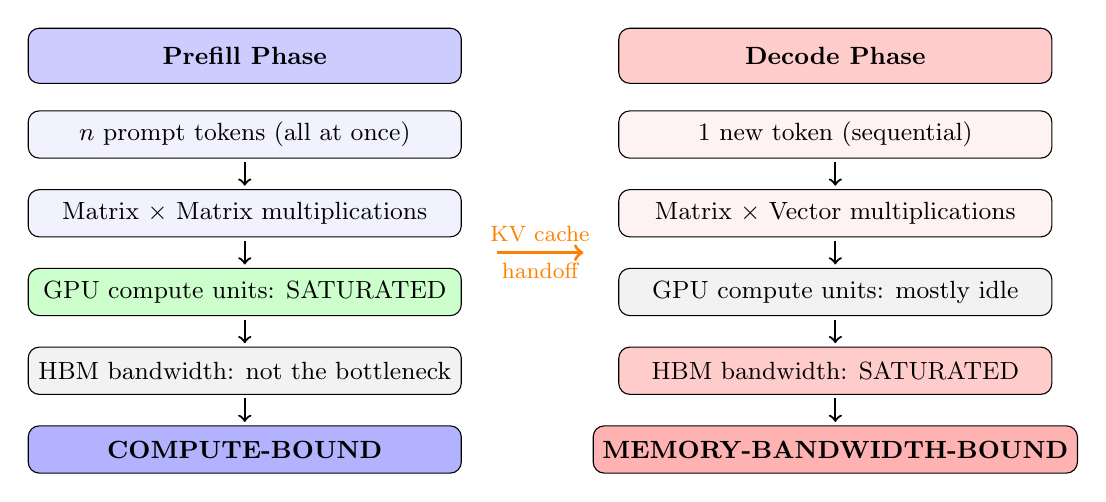
\begin{tikzpicture}[
    phase/.style={rectangle, rounded corners, draw, minimum width=5.5cm, minimum height=0.6cm, align=center, font=\small},
    header/.style={rectangle, rounded corners, draw, fill=#1, minimum width=5.5cm, minimum height=0.7cm, align=center, font=\small\bfseries},
    arr/.style={->, thick},
]
    % Prefill Phase
    \begin{scope}[shift={(0,0)}]
        \node[header=blue!20] (ph) at (0,5) {Prefill Phase};
        \node[phase, fill=blue!5] at (0,4) {$n$ prompt tokens (all at once)};
        \draw[arr] (0,3.65) -- (0,3.35);
        \node[phase, fill=blue!5] at (0,3) {Matrix $\times$ Matrix multiplications};
        \draw[arr] (0,2.65) -- (0,2.35);
        \node[phase, fill=green!20] at (0,2) {GPU compute units: SATURATED};
        \draw[arr] (0,1.65) -- (0,1.35);
        \node[phase, fill=gray!10] at (0,1) {HBM bandwidth: not the bottleneck};
        \draw[arr] (0,0.65) -- (0,0.35);
        \node[phase, fill=blue!30, font=\small\bfseries] at (0,0) {COMPUTE-BOUND};
    \end{scope}

    % Arrow between phases
    \draw[->, very thick, orange] (3.2,2.5) -- (4.3,2.5) node[midway, above, font=\footnotesize] {KV cache} node[midway, below, font=\footnotesize] {handoff};

    % Decode Phase
    \begin{scope}[shift={(7.5,0)}]
        \node[header=red!20] (dh) at (0,5) {Decode Phase};
        \node[phase, fill=red!5] at (0,4) {1 new token (sequential)};
        \draw[arr] (0,3.65) -- (0,3.35);
        \node[phase, fill=red!5] at (0,3) {Matrix $\times$ Vector multiplications};
        \draw[arr] (0,2.65) -- (0,2.35);
        \node[phase, fill=gray!10] at (0,2) {GPU compute units: mostly idle};
        \draw[arr] (0,1.65) -- (0,1.35);
        \node[phase, fill=red!20] at (0,1) {HBM bandwidth: SATURATED};
        \draw[arr] (0,0.65) -- (0,0.35);
        \node[phase, fill=red!30, font=\small\bfseries] at (0,0) {MEMORY-BANDWIDTH-BOUND};
    \end{scope}
\end{tikzpicture}
\caption{Prefill vs.\ Decode: two phases with opposite bottlenecks. Prefill processes all prompt tokens in parallel using matrix-matrix multiplications, saturating the GPU's compute units. Decode generates one token at a time using matrix-vector multiplications, saturating HBM bandwidth. The KV cache (Chapter~\ref{ch:kvcache}) is handed from prefill to decode so that key/value vectors need not be recomputed.}
\label{fig:prefill-vs-decode}
\end{figure}


\section{Summary}
\label{sec:ch2-summary}

We have built the transformer architecture from the ground up:
\begin{itemize}
    \item \textbf{Tokens} are sub-word integer IDs; the \textbf{embedding table} converts them to dense vectors.
    \item The \textbf{attention mechanism} lets each token gather information from other tokens by comparing queries against keys and reading from values. The $\sqrt{d_k}$ scaling prevents softmax saturation.
    \item \textbf{Multi-head attention} runs $h$ parallel attention heads with different learned projections, capturing multiple types of relationships.
    \item A \textbf{transformer block} combines attention (cross-position mixing) and a feed-forward network (per-position transformation), connected by a residual stream with layer normalization.
    \item \textbf{Stacking} $L$ blocks produces a deep model. Decoder-only architectures with causal masking enable left-to-right generation.
    \item \textbf{Autoregressive generation} produces one token at a time, with sampling strategies (temperature, top-$k$, top-$p$) controlling the trade-off between determinism and diversity.
    \item \textbf{Prefill} processes the prompt in parallel and is \textbf{compute-bound}. \textbf{Decode} generates tokens one at a time and is \textbf{memory-bandwidth-bound}. This asymmetry drives the design of every inference serving system.
\end{itemize}

\bigskip
\centerline{\rule{0.3\textwidth}{0.4pt}}
\bigskip

During the decode phase, each new token must attend to every previous token's key and value vectors. But those vectors don't change---recomputing them is pure waste. This observation leads to the single most important data structure in LLM serving.


% ===========================================================================
% Check Your Understanding
% ===========================================================================

\section*{Check Your Understanding}
\addcontentsline{toc}{section}{Check Your Understanding}

\emph{These questions start with recall and progress to conceptual reasoning. All are answerable from this chapter alone.}

\begin{enumerate}
    \item What are the three matrices in the scaled dot-product attention formula, and what role does each play?

    \item In a decoder-only transformer, why can token 5 attend to token 3 but not to token 7?

    \item Why does the attention mechanism divide by $\sqrt{d_k}$?

    \item Explain why the prefill phase is compute-bound and the decode phase is memory-bandwidth-bound. What is fundamentally different about the two computations?

    \item If you removed the residual connections from a transformer, the model would likely fail to train beyond a few layers. Why? What specific problem do residual connections solve, and how does the ``highway'' analogy from this chapter explain it?

    \item The FFN in each transformer block projects from $d_{\text{model}}$ up to $4 \times d_{\text{model}}$ and back down. Attention mixes information \emph{across} token positions, but the FFN operates on each position independently. If the FFN cannot see other tokens, what is it actually contributing to the model's computation? Why is it not redundant with attention?

    \item Suppose someone proposes a ``parallel autoregressive'' scheme: generate all output tokens simultaneously by running the full model once, taking the last-position output as token 1, the second-to-last as token 2, and so on. Explain precisely why this does not work---what mathematical property of the autoregressive factorization $P(t_1, \ldots, t_n) = \prod_i P(t_i \mid t_1, \ldots, t_{i-1})$ is violated, and why each factor's conditioning set matters.

    \item During decode, the model reads its full weight set (140\,GB for a 70B model) to produce a single token. A single A100 has 2\,TB/s of HBM bandwidth. Estimate how many tokens per second a single GPU can generate, and explain why increasing batch size helps---even though each request still needs one token at a time.

    \item The dot product $\mathbf{q}_i \cdot \mathbf{k}_j$ is symmetric: swapping the two vectors gives the same scalar. Yet attention scores are \emph{not} symmetric---token $i$ attending to token $j$ generally produces a different score than token $j$ attending to token $i$. Explain where the asymmetry comes from, and why the transformer's designers chose to keep the symmetric dot product rather than using an inherently asymmetric operator like additive attention.

    \item FlashAttention computes \emph{exactly} the same output as standard attention---it is not an approximation. Yet it reduces memory from $O(n^2)$ to $O(n)$ and runs significantly faster. If the mathematical result is identical, what is actually different? Why does changing the \emph{order} of computation matter so much, and what hardware property makes this possible?

    \item Consider the full inference pipeline: tokenization $\to$ embedding $\to$ $L$ transformer blocks $\to$ unembedding $\to$ softmax $\to$ sampling. Every component except the sampler is deterministic. Yet LLMs produce different responses to the same prompt. Where exactly does randomness enter the system, and why is this randomness \emph{necessary} rather than merely convenient? What would happen to long-form generation if you always picked the highest-probability token?
\end{enumerate}


\subsection*{Answers}

\begin{enumerate}
    \item $\mathbf{Q}$ (queries) represents what each token is looking for; $\mathbf{K}$ (keys) represents what each token advertises about itself; $\mathbf{V}$ (values) represents the information each token provides when attended to. The dot product $\mathbf{Q}\mathbf{K}^\top$ computes relevance scores; softmax normalizes them into weights; the weighted sum over $\mathbf{V}$ extracts the relevant information.

    \item The causal mask. In a decoder-only transformer, future positions are masked to $-\infty$ before softmax, so their attention weights become zero. This enforces the autoregressive property: each token can only depend on tokens at earlier (or equal) positions. Token 5 is at position 5, so it can attend to positions 1--5 but not position 7.

    \item Without scaling, the variance of the dot product $\mathbf{q}_i \cdot \mathbf{k}_j$ grows proportionally to $d_k$ (as shown in the variance derivation). For large $d_k$ (e.g., 128), the dot products become very large in magnitude, pushing softmax into a saturated regime where nearly all probability mass concentrates on one token. In this regime, gradients effectively vanish ($\partial\text{softmax}/\partial z_j \approx 0$), stalling learning. Dividing by $\sqrt{d_k}$ normalizes the variance back to a dimension-independent value, keeping softmax in a responsive range.

    \item \textbf{Prefill}: The model processes $n$ tokens in parallel. The dominant operations are matrix-matrix multiplications ($\mathbf{X}\mathbf{W}^Q$, $\mathbf{Q}\mathbf{K}^\top$, etc.)---large dense operations with high arithmetic intensity (FLOPs per byte of memory accessed). The GPU's compute units are fully utilized. \textbf{Decode}: The model processes one token at a time. The dominant operation is matrix-\emph{vector} multiplication---the full weight matrices must be read from HBM, but each is multiplied by a single vector, so the arithmetic intensity is very low. The GPU spends most of its time waiting for data from memory, not computing. The same weights are read per token either way, but prefill amortizes the read across $n$ tokens.

    \item Residual connections let each layer add its contribution to the residual stream rather than replacing it entirely. Without them, the output of layer $\ell$ \emph{is} the input to layer $\ell + 1$---the entire representation must be reconstructed at every layer. Gradients must propagate through a chain of transformations, vanishing or exploding over many layers. With residual connections, the gradient has a ``skip path'' that flows directly through the addition, keeping it well-behaved. The highway analogy: the residual stream is the highway carrying information from input to output; each layer is an off-ramp that reads from the highway, performs some computation, and adds its result back. If you remove the highway, every layer must perfectly encode \emph{everything} the later layers will need---an impossible burden for early layers.

    \item Attention determines \emph{which} positions are relevant to each other and transfers information between them, but the transferred information is a linear combination of value vectors---attention has no nonlinearity (except softmax, which only affects the \emph{weights}, not the \emph{values}). The FFN provides the model's \emph{nonlinear transformations}: it can detect feature combinations, activate learned knowledge patterns, and compute functions that linear mixing cannot. Think of it as the model's ``knowledge store''---early layers' FFNs learn syntactic patterns, later layers learn factual associations. The two sub-layers are complementary: attention mixes information across positions, and the FFN transforms information within each position.

    \item This fails because each factor $P(t_i \mid t_1, \ldots, t_{i-1})$ in the autoregressive factorization is conditioned on the \emph{actual tokens chosen} at earlier positions, not on a probability distribution over them. When you generate token 6, its distribution depends on which specific token was chosen as token 5. Generating all tokens simultaneously means each position conditions only on the \emph{input prompt}---it has no access to the other generated tokens. This computes $P(t_i \mid \text{prompt})$ independently for each $i$, which is a fundamentally different (and much weaker) distribution. The joint probability $\prod_i P(t_i \mid \text{prompt}) \neq \prod_i P(t_i \mid t_1, \ldots, t_{i-1})$ because the conditioning sets differ. Speculative decoding avoids this problem by having the large model \emph{verify} the draft tokens---it evaluates the true conditional distributions for all draft positions in one forward pass and accepts or rejects each token, preserving the exact autoregressive distribution.

    \item Reading 140\,GB of weights at 2\,TB/s takes $140/2000 = 0.07\,\text{s} = 70\,\text{ms}$ per token, giving roughly $1/0.07 \approx 14$ tokens/s for a single request. With a batch of $B$ requests, the model reads the weights \emph{once} and multiplies them against $B$ query vectors instead of one---the memory read (the bottleneck) is amortized. A batch of 32 produces 32 tokens per weight read, giving ${\sim}450$ tokens/s total throughput at nearly the same per-token latency. Batching converts the operation from matrix-vector (memory-bound) toward matrix-matrix (closer to compute-bound), increasing arithmetic intensity. The limit is GPU memory: the KV cache for all $B$ sequences must also fit in HBM alongside the weights.

    \item The asymmetry comes from the \emph{projections}, not the dot product. When token $i$ attends to token $j$, the model computes $\mathbf{q}_i \cdot \mathbf{k}_j = (\mathbf{x}_i\mathbf{W}^Q) \cdot (\mathbf{x}_j\mathbf{W}^K)$. When token $j$ attends to token $i$, it computes $\mathbf{q}_j \cdot \mathbf{k}_i = (\mathbf{x}_j\mathbf{W}^Q) \cdot (\mathbf{x}_i\mathbf{W}^K)$. These are different computations because the same token gets projected to a different vector depending on its \emph{role}: $\mathbf{x}_i$ becomes $\mathbf{x}_i\mathbf{W}^Q$ when asking but $\mathbf{x}_i\mathbf{W}^K$ when answering, and since $\mathbf{W}^Q \neq \mathbf{W}^K$, these are different vectors. Equivalently, the bilinear form $\mathbf{x}_i\mathbf{M}\mathbf{x}_j^\top$ where $\mathbf{M} = \mathbf{W}^Q{\mathbf{W}^K}^\top$ is not symmetric because $\mathbf{M} \neq \mathbf{M}^\top$ in general. The designers kept the dot product because it can be computed as a single matrix multiplication $\mathbf{Q}\mathbf{K}^\top$---a GEMM that saturates GPU tensor cores (high arithmetic intensity, compute-bound). Additive attention ($\mathbf{w}^\top \tanh(\mathbf{W}_1\mathbf{x}_i + \mathbf{W}_2\mathbf{x}_j)$) is inherently asymmetric but requires $n^2$ element-wise tanh operations that are memory-bandwidth-bound. The design insight: keep the fast symmetric operator and move all asymmetry into the learned projections that feed it.

    \item Standard attention materializes the full $n \times n$ score matrix in HBM (GPU main memory), which requires $O(n^2)$ memory and $O(n^2)$ HBM reads/writes. FlashAttention never materializes this matrix. Instead, it processes the input in blocks that fit in SRAM (the GPU's fast on-chip cache, ${\sim}20$\,MB on an A100 vs.\ 80\,GB of HBM), computing partial softmax results block by block and using the online softmax algorithm to combine them without ever needing the full matrix at once. The mathematical result is identical because online softmax is algebraically exact---it maintains running maximum and sum statistics that it corrects as new blocks arrive. The performance gain comes from the \emph{memory hierarchy}: SRAM is ${\sim}19$\,TB/s vs.\ HBM at ${\sim}2$\,TB/s on an A100. By keeping intermediate data in SRAM and only writing the final output to HBM, FlashAttention reduces HBM accesses from $O(n^2 d_k + n^2)$ to $O(n^2 d_k^2 / M)$ where $M$ is SRAM size. The key hardware property: GPUs have a massive gap between on-chip and off-chip bandwidth, so the order of computation---which data lives where, and for how long---matters enormously even when the total FLOPs are identical.

    \item Randomness enters at exactly one point: the sampling step, after softmax converts logits into a probability distribution. Temperature, top-$k$, and top-$p$ modify this distribution before sampling, but the draw itself is the sole source of non-determinism. This randomness is not just convenient---it is necessary for coherent long-form generation. Greedy decoding (always picking the highest-probability token) is deterministic but produces degenerate output: repetitive loops, generic safe phrasings, and inability to commit to a specific narrative direction. The reason is that the highest-probability token at each step is locally optimal but globally suboptimal---the model may assign 15\% to ``the'' and 12\% to ``a,'' and always choosing ``the'' pushes the model into a narrow corridor of high-frequency text. Sampling allows the model to explore diverse continuations that are collectively more likely under the true distribution than any single greedy path. Temperature controls the exploration-exploitation trade-off: low temperature ($\tau \to 0$) approaches greedy determinism, high temperature ($\tau \to \infty$) approaches uniform randomness. Crucially, sampling does not increase the computational cost at all---the full probability distribution must be computed regardless, and the sampling step itself is negligible.
\end{enumerate}
